\documentclass[conference]{IEEEtran}
\IEEEoverridecommandlockouts
%\bibliographystyle{IEEEtran}
%\bibliography{references}
\usepackage{cite}
\usepackage{amsmath,amssymb,amsfonts}
\PassOptionsToPackage{switch}{lineno} % Pass 'switch' option before loading
\usepackage{lineno}
\usepackage{tcolorbox}
\usepackage{graphicx}
\usepackage{blindtext}
\usepackage{flowchart}
\usepackage{mdframed}
\usepackage{tikz}
\usetikzlibrary{positioning,arrows,shapes.geometric,fit}
\usepackage{float}
\usepackage{minted}
% Ensure compatibility with TikZ
 % Uncomment only if necessary
 \tikzset{sharp corners/.append style={rounded corners=0pt}}
\usepackage{caption}
\usepackage{subcaption}
\usepackage{algorithm}
%\usepackage{algorithmic}
\usepackage{algpseudocode}
%\usepackage[switch]{lineno}
\usepackage{comment}
\usepackage{textcomp}
\usepackage[T1]{fontenc}
\usepackage{xcolor}
\def\BibTeX{{\rm B\kern-.05em{\sc i\kern-.025em b}\kern-.08em
    T\kern-.1667em\lower.7ex\hbox{E}\kern-.125emX}}
\begin{document}
\pagestyle{plain}
\title{Horses for Courses: Understanding System Development Parameters for the Matrix Multiplication Kernel
 \\
}
\begin{comment}
\author{\IEEEauthorblockN{Vyuhita Bonthu}
\IEEEauthorblockA{\textit{Indian Institute of Technology Dharwad, India} \\
\textit{212011001@iitdh.ac.in}}
\and
\IEEEauthorblockN{Nikhil Hegde}
\IEEEauthorblockA{\textit{Indian Institute of technology Dharwad, India} \\
\textit{nikhilh@iitdh.ac.in}}
}
\end{comment}
\maketitle

\begin{abstract}
Matrix multiplication is a fundamental kernel in domains ranging from machine learning to high-performance computing to benchmarking computer architectures. Developers devote significant time and effort to optimize matrix multiplication kernels. In this paper, we present a systematic study of 
 the performance, speed of development, and energy consumption of multiple flavours of implementations of the matrix multiplication kernel on multicore, manycore, SIMD-, and accelerator- based hardware. We implement hybrid-parallel codes which are a mix of hand-optimized and tool-generated codes and compare them with standard implementations of the matrix multiplication kernel. For various matrix sizes, performance, development effort, and energy consumption of AVX, AVX2, Cilk, OMP, CUDA, and hybrid parallel codes are measured. 
 We implement the recursive matrix multiplication algorithm using task-parallel paradigms available for multicore systems. We make the recursion base case implementation tunable and plug hand-optimized AVX, AVX2, and CUDA code. In some implementation versions, the recursive algorithm is implemented using a code generation tool, which left the recursion base case empty to allow for plugging in of hand-optimized code. We then plug hand-optimized kernel in such implementations. Scalability experiments with different programming models on CPUs, multiple GPUs, Arm server on cloud, and Jetson Nano show that  CUDA implementations not only offer the lowest latency but also are energy efficient in a multi-GPU setting, where the work is distributed. Interestingly, for extended-precision codes, we observe that tool-generated code augmented with hand-optimized CUDA kernel executed on multi-GPU systems performs better than native CUDA code in all aspects of latency, development speed, and energy consumption. 
\end{abstract}


%\end{IEEEkeywords}

\section{Introduction}
Matrix Multiplication is a central operation in algorithms that are used every day now. E.g., training a model in Machine learning, displaying sharper images in Computer Graphics, predicting weather patterns in Scientific Computing, analysis of Social Network relations, studying cache designs in Computer Architecture, benchmarking the speed of a Supercomputer are a few important examples where matrix multiplication is employed. Improving the speed of computation of matrix multiplication has been the focus of mathematicians and computer scientists for many decades. Algorithmic improvements that yield lesser number of multiply-add operations~\cite{huss1996implementation}, improvements in scheduling of those operations to yield lesser number of memory accesses to the slow memory in modern computing systems with hierarchical memory~\cite{low2004api,van1997summa}, provisioning of dedicated hardware for simultaneous execution of several such operations form the broad spectrum of developments~\cite{10.1137/140993478}. Orthogonally, researchers have created abstractions and tools for developers to {\em quickly} produce fast matrix multiplication implementations: dedicated APIs for matrix multiplication in library-based development environment~\cite{MKL,Alpatov1997PLAPACKPL,goto2008high,choi1992scalapack,anderson1999lapack,libflame}, compilers to effectively map the operations to underlying hardware~\cite{ikarashi2022exocompilation}, and programming systems to abstract the specification of computation from orchestrating the computation on underlying (often) complex hardware~\cite{ragan2013halide}. This paper focuses on various factors 
 involved in system development ---development to deployment on specific systems--of matrix multiplication in an attempt to understand the trade-offs involved. Specifically, on a variety of hardware, such as DNN accelerators, GPUs, x86- and Arm-based multicore CPU servers, performance characteristics at different scales within the system are considered: i) within a core: SIMD/vectorized and multithreaded codes, ii)across cores: shared-memory parallel programming models using Cilk, OpenMP tasks, iii) hybrid codes i.e. CPU+GPU including automatically generated codes. Latency, energy consumed, and  speed of code development are measured for single- and double-precision data to understand the tradeoffs of execution time vs. \{precision, energy consumption\}, precision vs. energy consumption, speed of code development vs. \{energy consumption, execution time, and precision\}. The goal is to help application developers make an informed choice of the workhorse (system with appropriate programming abstraction and tools) for deploying their applications, which have matrix- multiplication as the underlying kernel. 
 
Modern computing systems provision for parallelism within a core, across cores, across a host within the same compute node hosting one or more `devices' or accelerators, and across a host with multiple nodes. A single optimized implementation that delivers the same level of performance with system configurations of different parallelism levels is challenging.  Developers dedicate significant time and effort to optimize matrix multiplication kernels to squeeze out every ounce of performance from the hardware resources available. We create `reasonably' efficient implementations of matrix multiplication {\em quickly} with the help of a tool, D2P~\cite{hegde2019d2p}, that produces parallel code exploiting parallelism across cores and across hosts on multiple compute nodes. Furthermore, D2P provisions for exploiting parallelism within a core and in a node with host-device mode of computing. This {\em elastic} parallel code is created from a specification, which we develop assuming dense matrix computation and a recursive divide-conquer (non-Strassen) matrix multiplication algorithm. A noteworthy feature of the elastic code is that the recursion base case is left empty to allow for optimized kernels to be plugged-in. Consequently, we plug in hand-tuned, optimized kernels (CUDA, AVX, Arm Neon, locality-optimized) and augment to create efficient, performance portable matrix multiplication implementations quickly. It is important to note that the development of hand-tuned optimized code is a one-time effort (often available) and 
 plugging-in and deploying augmented code on different systems is relatively easier.

 
%Therefore, To make the most of the underlying hardware capabilities, they employ SIMD parallelism, which includes the AVX and AVX2 instruction sets. They also use parallelizing constructs to optimize the performance of each core. 
%Better optimization requires in-depth analysis and profiling to comprehend trade-offs between latency, cost, energy consumption, and development speed.
% Gap?
%Our focus is on addressing the gap i.e., the need for a comprehensive analysis of the various aspects mentioned earlier.

Figure~\ref{fig:1} shows performance comparison of the augmented code 
 (indicated as hybrid code) and native CUDA-C code for multiplying two matrices. The hybrid code is a mix of MPI+Cilk+CUDA-C code. Interestingly, we see that in a compute node with multiple GPU cards, native CUDA-C implementation executes slower compared to the hybrid code. 
% Profiling details showed that the hybrid multi-GPU CUDA implementation spent only 27.5\% on kernel execution and the rest of 72.5\% of execution time on memory transfer. In contrast, the Native Single GPU and Native Multi-GPU implementations spend 98\% of their execution time on kernel execution and only 2\% on memory transfer. This large difference in time allocation explains why the hybrid code runs faster.
Performance counters from NVIDIA Nsight Compute indicate why the hybrid code performs better than the native code. The hybrid code records nearly 56 million DRAM active cycles, whereas the native code displays a much higher 9.54 billion cycles. The hybrid code also achieves better overall DRAM throughput (8.24\% versus 5.11\%) and memory throughput (21.95\% compared to 18.54\%). The  L1 cache throughput for hybrid code is higher than native code (43.32\% versus 37.08\%) but the hybrid code records comparatively lesser L2 cache throughput (4.09\% compared to 4.73\%). On the other hand, the registers per thread used for hybrid code (36) are lesser than native code (46), leading to greater parallelism . With slightly improved GPU occupancy (100.49\% versus 100.13\%), the hybrid code maximizes resource utilization more effectively, leading to faster execution and superior performance overall.
 We attribute this to the dynamic parallelism created in hybrid code, which is able to utilize the additional GPU resources efficiently. The recursion base cases (with CUDA kernels) in the hybrid code are independent tasks that get executed with the help of distinct MPI ranks. Note that both hybrid code (in the recursion base case) and native code use the same optimized CUDA kernel for matrix multiplication.
 This experiment shows that performance portability across multiple GPU cards is achievable with minimal programmer effort and surprisingly, tool-produced code can be faster than hand-optimized code. Is the performance portability free of cost? does data precision have an impact on performance and/or energy consumption? to understand these, we do a systematic analysis of the performance (execution time), development speed, and energy consumption of different flavours of matrix multiplication kernel implementations on a variety of systems, including Jetson Nano and cloud-based server instances. 
%We aim to identify each implementation's efficiency gains and tradeoffs across various hardware platforms. 
%In this study, we implement and conduct a thorough evaluation of hand-optimized versions, tool-generated implementations, and library-based solutions. 
%We test the performance, development speed, and energy consumption of SIMD codes such as AVX and AVX2, CPU-parallel codes like Cilk and OpenMP (OMP), CUDA for using the GPU card, and tool-generated hybrid parallel codes for various matrix sizes. We improve the recursive matrix multiplication algorithm by implementing multicore-specific Cilk and OMP parallelizing constructs. We used D2P to generate MPI and Cilk based hybrid code implementation by providing recursive algorithm specifications. The tool-generated code has the empty recursion base case, making it performance portable. We plug the hand-optimised AVX, AVX2 and CUDA codes into the base case.
The key contributions are:
%\begin{figure*}[h!]
%  \centering
%  \includegraphics[width=0.9\linewidth]{3dPlot.png}
%  \vspace{-0.8em}
%  \caption{Comparison of hand-optimized and tool-generated implementations of various programming models for both precisions.}
%  \label{fig:3d}
%\end{figure*}
\begin{itemize}
 
    \item We create specifications for recursive matrix multiplication algorithm and produce corresponding hybrid-parallel code.  
    \item We create a number of matrix multiplication implementations, including AVX256, AVX512, Arm Neon, OpenMP, Cilk, Jetson Nano, CUDA-C, Open BLAS-based, Tensorflow, and Pytorch based codes. We plug-in some of these codes into the recursion base case to produce efficient hybrid-parallel code. 
    \item we measure and analyze performance, energy consumed, precision and speed of development to understand trade-offs involved in multiplying matrices with different precision data, on systems at different scales, with different programming systems, under different energy consumption scenarios. 
\end{itemize}
\begin{figure}[H]
  \centering
  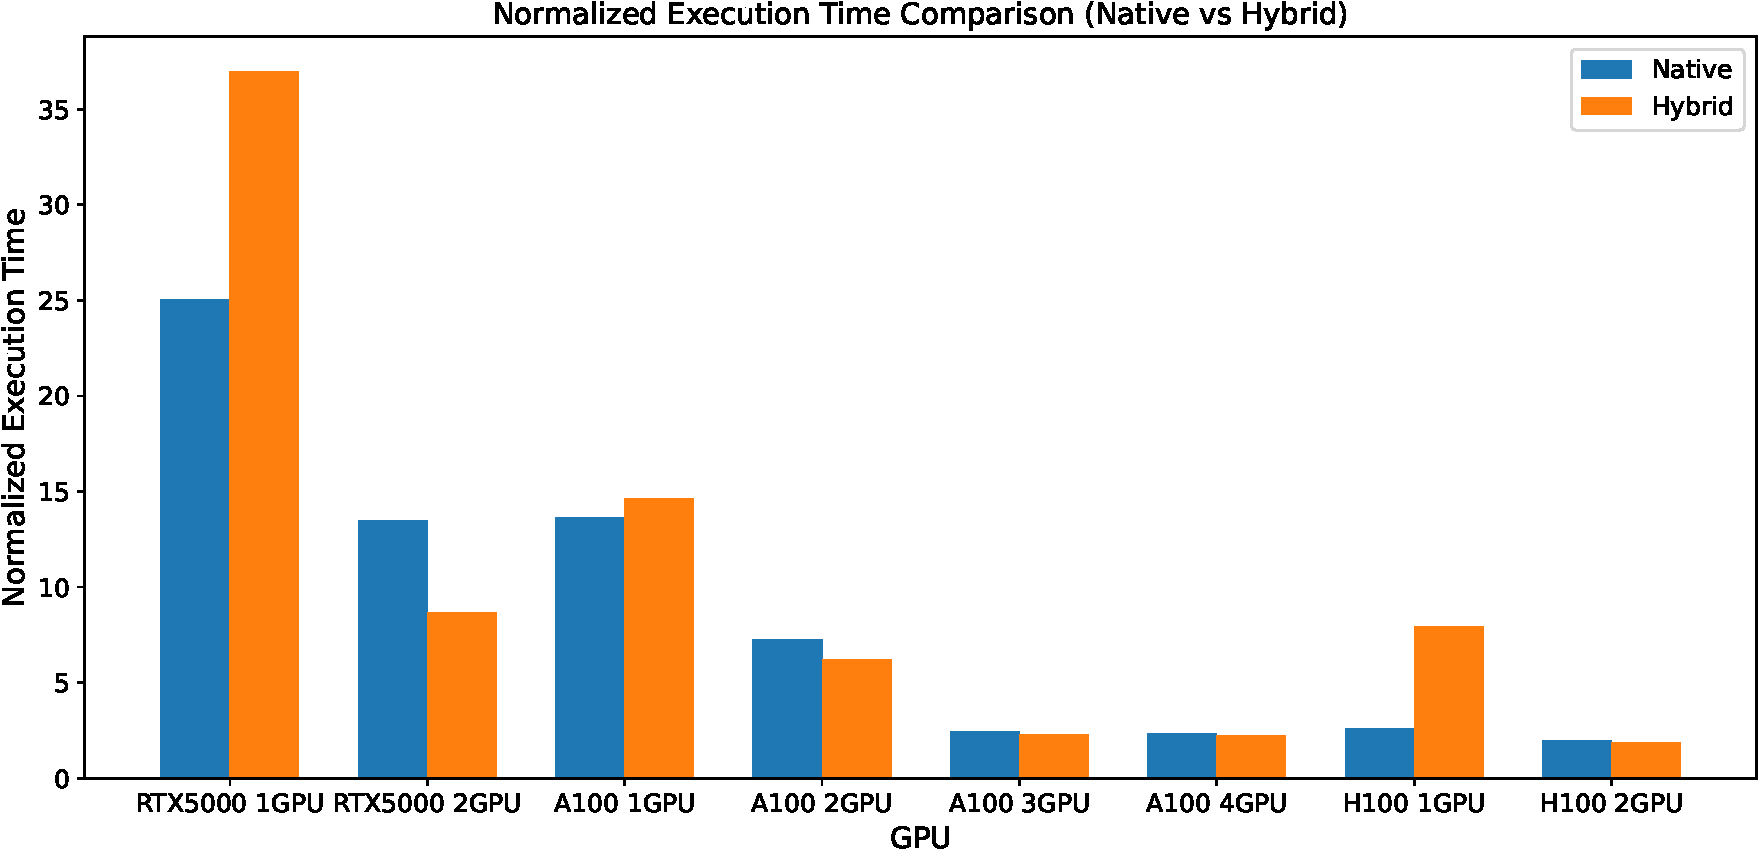
\includegraphics[width=1.0\linewidth, height=0.70\linewidth ]{Images/DiffHardware -crop.pdf}
  %\vspace{-0.8em}
  \caption{Native CUDA-C vs. Augmented CUDA-C comparison.}
  \label{fig:1}
\end{figure}

Tests across various systems show that overall, CUDA implementations executing on multiple GPUs deliver the best performance, offering the lowest latency. W.r.t. energy consumption of distributed workloads, surprisingly, codes executing on RTX5000 GPUs show that energy consumption get smaller with work distributed across available cards. In contrast, energy consumption increase with work distributed across available A100 and H100 GPUs.  As expected, increasing precision from single- to double- floating point computation is associated with longer execution time, which in turn is associated with increased energy consumption. The cuda codes on Jetson Nano w.r.t to performance %also take longer execution time and consume more energy for double precision than single precision. %jetson nano to a100, ARM and PNK, ARM VM and BM, omp & cilk on ARM
are 7.5x slower than RTX5000, 28.48x slower than A100 and 37.47x slower than H100. And w.r.t. energy consumption, Jetson Nano consumes 5.2x less energy than RTX5000, 10.49x less energy than A100 and 8.4x less energy than H100. 
Interestingly, for CPU Parallel codes like OMP and Cilk, OMP and Cilk on x86 are 1.4x and approximately 1.5x slower than runs on ARM for both single- and double- precision.
%Tests on AVX256 and AVX512 codes on RTX5000 show that AVX512 offers better performance and energy efficiency than AVX256 in both the precisions, w.r.t the Hybrid -AVX256 and -AVX512 codes, the performance is better for hybrid AVX512 but not energy efficient, and interestingly Hybrid AVX512 \& AVX512 codes deliver better performance than Native AVX256 \& AVX512  codes but energy consumption-wise Native codes are more energy efficient in both single and double precisions.
The SIMD codes on ARM, w.r.t. performance, are 1.9x slower than x86, whereas Hybrid SIMD codes on ARM are 20x slower than Hybrid SIMD x86 for single precision.
For double precision, Native SIMD on ARM is 4x slower than x86, whereas SIMD codes on ARM are 23.4x slower than Hybrid SIMD x86 for single precision.
A similar trend is observed in SIMD codes on ARM system w.r.t precision, additionally, native SIMD codes consistently perform better than Hybrid SIMD codes in single and double precisions. 
Also, ARM virtual machine instance SIMD codes are 1x slower than ARM Bare metal instances.
Tests on Colab for TPU and GPU usage using TensorFlow and PyTorch show that runs on TPU perform well when compared to GPU. TensorFlow code using TPU is faster than PyTorch using TPU for single and double precisions. In contrast, PyTorch GPU code is faster than TensorFlow GPU code.
Due to the limited access to performance counters on cloud-based instances and Google Colab, energy consumption was not measured.
%Experiments with different programming models on Arm-based and x86-based CPU-only servers, CPU-GPU servers with multiple GPU cards, and Jetson Nano demonstrate that CUDA implementations provide the lowest latency and are the most energy-efficient in a multi-GPU scenario with distributed work. 
%We see trade-offs across various CPU and GPU-based implementations demonstrated in the figure\ref{fig:1} below.
%We observe that double precision take more energy and are slower compared to single precision. We also see that using multiple GPUs can improve latency as the work can be disributed and computed simultaneously. we also observe that d2p+AVX512d seems to consume more energy than d2p+AVX256d for both single and double precision.
%Specifically, for double precision codes, we find that tool-generated code integrated with a manually optimised kernel on a multiple GPU setting performs better than native CUDA code in terms of latency, development speed, and energy consumption.
%We also see many other contrasting behaviors in figure \ref{fig:1}. A detailed discussion will be presented in the Result and Analysis section.

The remainder of the paper is organised as follows: Section 2 lays out the background of producing parallel code and augmenting; Section 3 discusses the analysis of system development parameters, Section 4 provides related work, and lastly, Section 5 concludes.

\section{Producing Parallel Code and Augmenting}
\begin{table*}[t]
%\begin{wraptable}{l}{0.5\textwidth}

\centering
\vspace{-0.8em}
\caption{Algorithm (left), Specification (right)}
\label{tab:mytable}
\begin{minipage}{.45\linewidth}
\centering
%\begin{table}[H]
%\parbox[t]{\linewidth}{\caption{Algorithm}}
\begin{small}
%\textbf{Algorithm}
\centering
\vspace{10pt}
$\left[\begin{array}{ll}
A_{00} & A_{01} \\
A_{10} & A_{11}
\end{array}\right] \times\left[\begin{array}{ll}
B_{00} & B_{01} \\
B_{10} & B_{11}
\end{array}\right]=\left[\begin{array}{ll}
A_{00} B_{00}+A_{01} B_{10} & A_{00} B_{01}+A_{01} B_{11} \\
A_{10} B_{00}+A_{11} B_{10} & A_{10} B_{01}+A_{11} B_{11}
\end{array}\right]$

\end{small}
%\end{table}
\end{minipage}%
\begin{minipage}{.45\linewidth}
\centering
%\begin{small}
%    \textbf{Specification}
%\end{small}
\begin{small}
\begin{verbatim}
A(<x,y,z>)
Parallel: A(<x00 y00 z00>) A(<x01 y00 z01>) 
         A(<x10 y10 z00>) A(<x11 y10 z01>)
Parallel: A(<x00 y01 z10>) A(<x01 y01 z11>) 
         A(<x10 y11 z10>) A(<x11 y11 z11>)
\end{verbatim}
\end{small}

\end{minipage}
\end{table*}

%\end{wraptable}
%\clearpage

Table~\ref{tab:mytable} presents a recursive approach and the corresponding specification to compute the product of two matrices $A$ and $B$. The approach on the left partitions the matrices into block matrices with four blocks of roughly equal size. It then computes the product of blocks to form the final product. This divide-conquer approach is represented with a method specification on the right. The specification requires that the first parameter of a method is the write parameter, and remaining are the read parameters. Hence, the recursive method represented as \texttt{A}  computes the product of two matrices \texttt{y}, and \texttt{z} and adds the result to the data stored in matrix \texttt{x}.  Essentially method \texttt{A} represents a multiply-add operation. The details of symbols \texttt{<}, \texttt{>}, blankspace or comma to separate arguments can be ignored and have no special meaning. The keyword \texttt{Parallel} is an annotation that tells that all the method calls on the same line may be executed in parallel. As we can see, there is a one-to-one correspondence between the specification and the divide-conquer approach on the left. The specification 
 shows further details indicating multiplication of \texttt{$y_{ij}$} and \texttt{$z_{ij}$} and adding  the result to \texttt{$x_{ij}$}. 
 Note that the base case of recursive method is not part of the specification. Also, note that for matrix sizes that are powers of two, the method works very well without extensions. In the code that is emitted from this specification, the base case implementation is left blank and is expected to be augmented with optimized kernels such as SIMD codes, CUDA kernels, or locality optimized codes.  

Starting from the specification, the MPI+Cilk code generation requires  parallelism inference, data decomposition, task creation, and communication insertion. Importantly, the generated code will be correct only if the specification corresponding to the algorithm satisfies the {\em inclusive} and {\em intersection} properties. We omit these and provide a system-level overview here and refer the readers to~\cite{hegde2019d2p} for details. The specification for recursive matrix multiplication can be written in multiple ways e.g., with the help of two recursive methods \texttt{A} and \texttt{B}, where method \texttt{A} implements the addition and method \texttt{B} implements the multiplication. However, some specifications may lead to inefficiencies when temporaries are used and some may not satisfy the inclusive and intersection properties. ~\cite{hegde2019d2p} showed the existence of those properties in all Dynamic Programming (DP) algorithms. Whereas, in this paper we consider a flavor of matrix multiplication algorithm, create the corresponding spec and generate efficient hybrid parallel code. Figure~\ref{fig:workflow} illustrates the system overview. The specification is input to D2P to generate 
 MPI+Cilk parallel code. This code has recursive method implementations with empty recursion base case, which is filled by the programmers. The resulting augmented code is a hybrid-parallel code that is executed on SIMD, multicore, manycore, and GPUs.  % d2p paper
\begin{figure}[h]
    \centering
    
\tikzset{
    >=stealth',
    % Specifications for style of nodes:
    base/.style = {
            rectangle,
            rounded corners,
            draw=black,
            minimum width=1in,
            minimum height=0.5in,
            text centered
            % ,
            % font=\sffamily
        },
    every node/.style={
            inner sep=.25cm,
            fill=white
            % ,
            % font=\sffamily
        }
}
\tikzstyle{XOR} = [draw,circle]
\tikzstyle{line} = [draw, very thick, color=black!50, -latex']


\begin{tikzpicture}[node distance=0.5cm, align=center]
    \node[base](spec){Specification};
    \node[base,below = of spec](d2p){D2P};
    \node[base,below = of d2p](gen){MPI + Cilk \\ implementation \\ with gaps};
    \node[XOR,inner sep=0, right = of gen](xor){\huge +};
    \node[base,right = of xor](usr){Optimized kernels\\  like AVX, \\ AVX2 and CUDA-C};
    \node[base,below = of xor, yshift=-0.5cm](done){Completed \\ implementation};
    
	\path [line] (spec) -- (d2p);
	\path [line] (d2p) -- (gen);
	\path [line] (gen) -- (xor);
	\path [line] (usr) -- (xor);
    \path [line] (xor) -- (done);
\end{tikzpicture}

    \caption{System overview}
    \label{fig:workflow}
\end{figure}
 
%\begin{mdframed}[linewidth=0.10pt,linecolor=black]
\begin{figure}[h]
\begin{minted}[fontsize=\footnotesize]{c}
void A( /* Method Signature */ ) {
    if ((x->coords[0] == x->coords[2]) 
    && (x->coords[1] == x->coords[3])) {   
    \end{minted}
    \vspace{-3mm}
\begin{tcolorbox}[colback=white, boxrule=0.5pt, sharp corners,title= Optimized terminating case with AVX.  ]
\begin{minted}[fontsize=\footnotesize]{c}
 // Loop over rows of A
    for (int i = 0; i < size; i++) {
        // Loop over columns of B
        for (int j = 0; j < size; j++) {
        // Initialize the result vector to zero
            __m256i result = _mm256
                             _setzero_si256();
            // (process 8 elements at a time)
            for (int k = 0; k < size; k += 8) {
                // Load 8 elements from B and C
                __m256i b = _mm256_loadu_si256
                ((__m256i*)&B[i * size + k]);
                //similarly for c
                // Multiply and accumulate
                result = _mm256_add_epi32(result
                , _mm256_mullo_epi32(b, c));
            }
            //Accumulate result into A
        }
    }
    \end{minted}
\end{tcolorbox}
\begin{minted}[fontsize=\footnotesize]{c}   
     // Auto Generated Code to handle
    A_unroll(&x00, xData, parentTileIDx * 4 + 0,
    &y00, yData, parentTileIDy * 4 + 0, &z00, 
    zData, parentTileIDz * 4 + 0,
    callStackDepth + 1);//similarly for x01,x10,x11  
    A_unroll(&x00, xData, parentTileIDx  * 4 + 0,
    &y01, yData,parentTileIDy * 4 + 1, &z10,
    zData, parentTileIDz  * 4 + 2,
    callStackDepth + 1);//similarly for x01,x10,x11
}
\end{minted}
 \caption{Augmenting with AVX code.}
    \label{fig:d2p_avx}
\end{figure}
%\end{mdframed}


\begin{figure}[h]
\begin{minted}[fontsize=\footnotesize]{c}
void A( /* Method Signature */ ) {
  if (x->coords[0] == x->coords[2]) 
  && (x->coords[1] == x->coords[3])) {  
  \end{minted}
  \vspace{-3mm}
\begin{tcolorbox}[colback=white, boxrule=0.5pt, sharp corners, title= Optimized terminating case with NEON. ]
\begin{minted}[fontsize=\footnotesize]{c}
 // Loop over rows of A
  for (int i = 0; i < size; i++) {
    // Loop over columns of B
    for (int j = 0; j < size; j++) {
      // Initialize the result vector to zero
      float32x4_t result = 
                      vdupq_n_f32(0.0f);
      // process 4 elements at a time)
      for (int k = 0; k < size; k += 4) {
        // Load 4 elements from B and C
        float32x4_t b = vld1q_f32
                          (&B[i * size + k]);
        // Similarly for C and then Multiply
        //and accumulate
        result = vmlaq_f32(result, b, c);
      }
      // Accumulate the result into A
    }
  }
\end{minted}
\end{tcolorbox}
\begin{minted}[fontsize=\footnotesize]{c}
// auto-generated code to handle
  A_unroll(&x00, xData, parentTileIDx * 4 + 0,
  &y00, yData, parentTileIDy * 4 + 0, &z00, 
  zData, parentTileIDz * 4 + 0,
  callStackDepth + 1);//similarly for x01,x10,x11
  A_unroll(&x00, xData, parentTileIDx * 4 + 0,
  &y01, yData,parentTileIDy * 4 + 1, &z10,
  zData, parentTileIDz * 4 + 2,
  callStackDepth + 1);//similarly for x01,x10,x11
}
\end{minted}
\caption{Augmenting with Arm Neon code.}
    \label{fig:d2p_NEON}
\end{figure}

Figures~\ref{fig:d2p_avx} and ~\ref{fig:d2p_NEON} show how handwritten SIMD codes for x86 and Arm systems are integrated with D2P generated code to produce hybrid code. We use intrinsics---C-style functions provided to manipulate the vector registers without writing assembly code---available from Intel and Arm. The same technique is applied to create a number of flavors of hybrid parallel code where the base case implementations to multiply two matrices (of smaller sizes) are different. The below list shows a complete list of different flavors of matrix multiplication implementations:
\begin{itemize}
\item \texttt{d2p\_avx, d2p\_avx2, avx, avx2}: code using the 256-bit and 512-bit vector registers on x86 architecture. Meant for execution on multicores, manycores across compute nodes.
\item \texttt{d2p\_neon, neon}: code using Arm's Neon vector registers. Meant for execution on multicores, manycores across compute nodes.
\item \texttt{d2p\_cuda, cuda}: code using single GPU to accelerate matrix multiplication. Meant for execution on GPU servers.
\item \texttt{d2p\_cublas, cublas}: code using single GPU and a BLAS-like library API available to multiply matrices. Meant for execution on GPU servers.
\item \texttt{d2p\_cudamultigpu, cudamultigpu}: code using multiple GPUs to accelerate matrix multiplication. Meant for execution on GPU servers.
\item \texttt{omp} recursive implementation of matrix multiplication using OpenMP tasks. Meant for execution on multicore CPU servers.
\item \texttt{Cilk} recursive implementation of matrix multiplication using Cilk. Meant for execution on multicore CPU servers.
\item \texttt{pytorch\_cpu, pytorch\_gpu, pytorch\_tpu} implementation using the Pytorch framework on multicore CPU, GPU, and TPU.
\item \texttt{tensorflow\_cpu, tensorflow\_gpu, tensorflow\_tpu} implementation using the Tensorflow framework on multicore CPU, GPU, and TPU.
\item \texttt{jetson\_nano} iterative implementation of matrix multiplication using CUDA on Jetson nano.
\end{itemize}

In the above list, flavors that do not have \texttt{d2p\_} prefix are implementations that are not hybrid parallel i.e. are not codes generated by D2P. They are handwritten optimized implementations using recursive algorithm.  Also, each of the above flavors have two sub-flavors one each corresponding to single- and double-precision data. 



\section{Analysis of System Development Parameters}
We consider the most significant parameters involved in the system development: performance in terms of execution time, energy consumption, speed of implementing the code. These three broadly summarize the cost of ownership of a particular implementation. Speed of implementation is a metric that is custom defined for software systems e.g. based on the number of features implemented, based on number of lines of code written, etc. Here, we go with a broad notion that vector codes (using intrinsics or assembly) are the slowest and most difficult to develop and tool generated codes are the fastest and least time consuming to develop. In particular the following is considered w.r.t. speed of development: 
$\texttt{SIMD} < \texttt{tiled} < \texttt{GPU} \leq \texttt{jetson\_nano} \leq \texttt{OMP} \leq \texttt{Cilk} < \texttt{pytorch} \leq \texttt{tensorflow} < \texttt{d2pxx}$. 
Cost of ownership~\cite{barroso2019datacenter} is usually defined for data center designs. We introduce it here as a metric for evaluating the efficiency of matrix multiplication as deployed. Considering the pervasiveness of running Gen-AI workloads (and the matrix-multiplication operation running underneath) on systems on Cloud-based, on premise-servers, HPC clusters, workstations, edge devices, and on personal computing systems, we believe the following choice of hardware and the implementation flavors mentioned earlier help developers and end-users to decide on a suitable system, framework, and precision to develop and deploy their applications.   
\begin{figure*}[ht!]
  \centering
 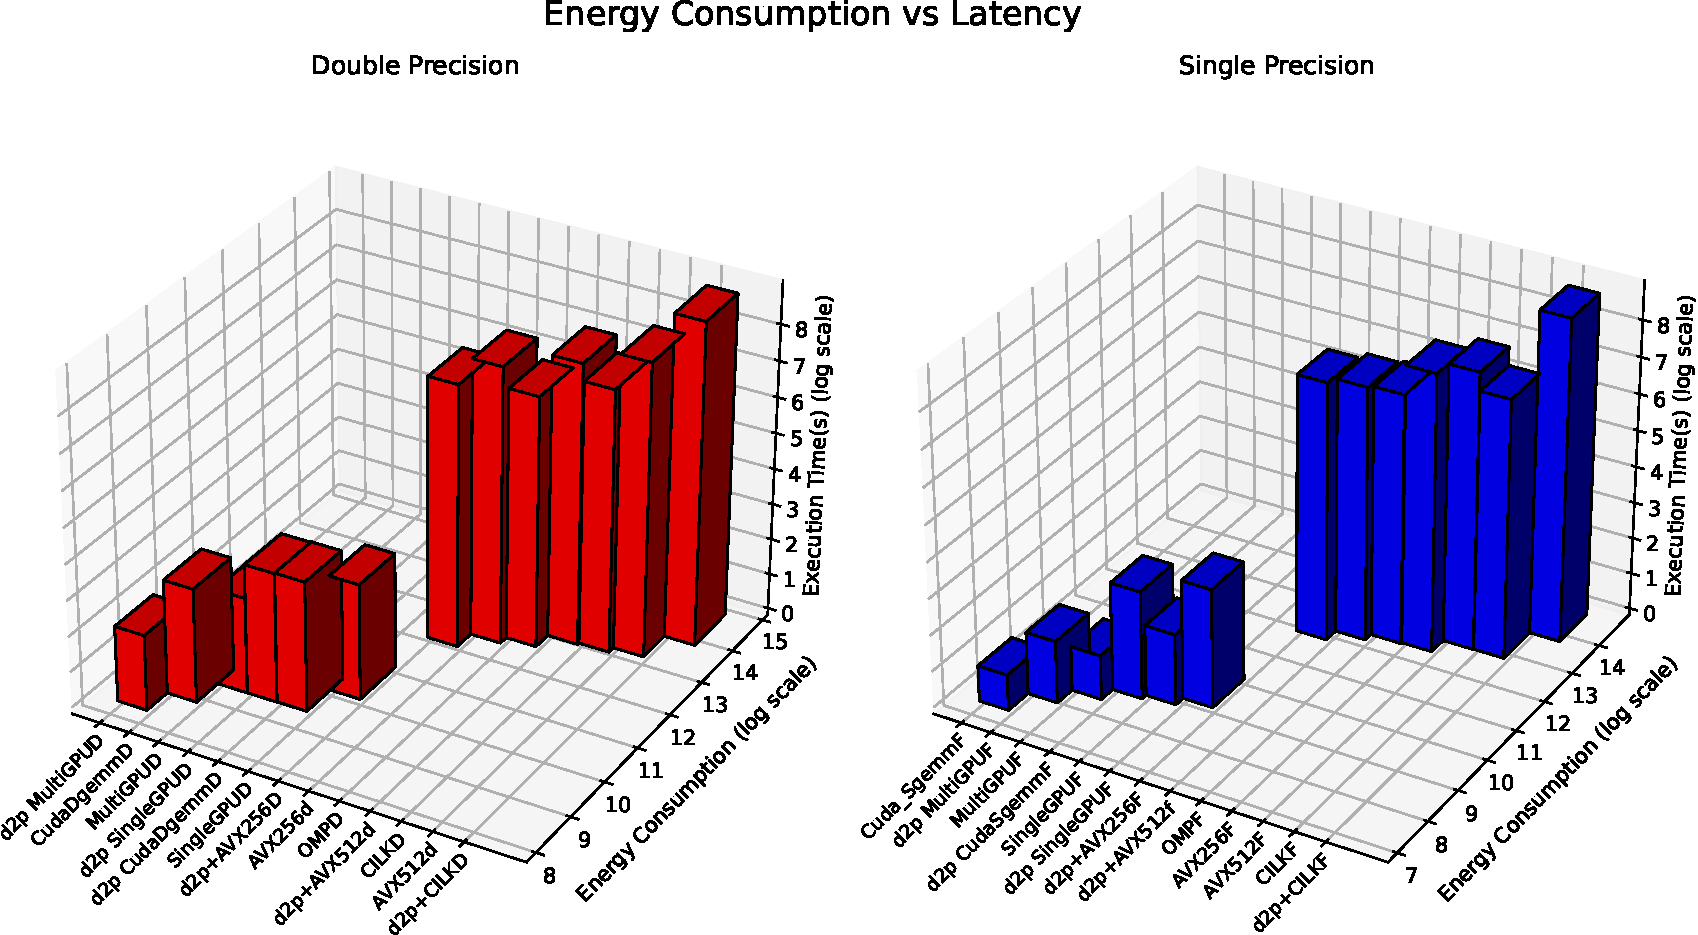
\includegraphics[width=0.9\linewidth]{Images/3d-crop.pdf}
  \vspace{-0.8em}
  \caption{Energy-Execution\_Time-speed\_of\_development plots 
for different implementations with single- and double-precison inputs.}
  \label{fig:3d}
\end{figure*}
\subsection{System Configuration}
We have conducted tests on multiple systems: 
\begin{itemize}
\item Intel(R) Xeon(R) Gold 6240C CPU, 36 physical cores in total in a 2-socket configuration, 2.2MiB L1 cache, 36MiB L2 cache and 49.5MiB L3 cache. Core base frequency is kept at 2.60GHz and the TDP is 150W (Thermal Design Power, which is the average power in watts, that the processor consumes while running at base frequency with all cores active under a complex workload). This system also has two NVIDIA QUADRO RTX 5000 GPUs, each with 16 GB memory and 3,072 CUDA cores, with a maximum power draw of 230W. Evaluated SIMD, CPU-only, Tensorflow-GPU, Tensorflow-CPU, Pytorch-CPU, Pytorch-GPU, BLAS-based, CUDA BLAS based codes on this server. Hybrid parallel codes are also evaluated on this server. 
\item A cluster of two compute nodes and a master node. One of the compute nodes has four A100 cards and the other has two H100 cards. Each with a memory capacity of 80GB. Single GPU and Multigpu codes including using CUDA BLAS libraries are evaluated on these servers. 
\item Jetson Nano has 128 Cuda cores, each with a memory of 4GB and a maximum power draw of 10W.
\item We also employed an AWS Graviton3 processor \texttt{c16\_large}, with 64 cores. This is a cloud-based instance offering VM environment. We have used this to run Arm Neon codes. We have also run experiments on \texttt{c16\_metal}, the baremetal version and observed that the overhead of VM environment is insignificant.
\item Google Colab to test TPU codes in TensorFlow and PyTorch frameworks.
\end{itemize}

During execution, we unrolled the recursion to a depth of 1 to create parallellism for tasks in D2P. This resulted in 8 tasks and we used 4 processes (MPI ranks) to measure the parameters mentioned. 4 processes were considered after we empirically found that the 4-process configuration yielded the best performance (lowest latency). 
We have used perf events for measuring the energy consumption (in Joules) of CPU-based implementations. For measuring GPU energy consumption, we have mainly used Nvidia-smi to monitor GPU power consumption, multiplied it with total execution time to obtain energy consumed by the GPU, and perf to measure the CPU’s overall package energy. Then, we added both energies to calculate the total energy consumed by the GPU and CPU
during the code’s execution.
Our attempt to measure energy consumption on the
the ARM instance on AWS was unsuccessful due to the limited access to performance counters.
\begin{figure*}[htbp]
\centering
\begin{tabular}{cc}
    \begin{minipage}{0.45\linewidth}
        \centering
        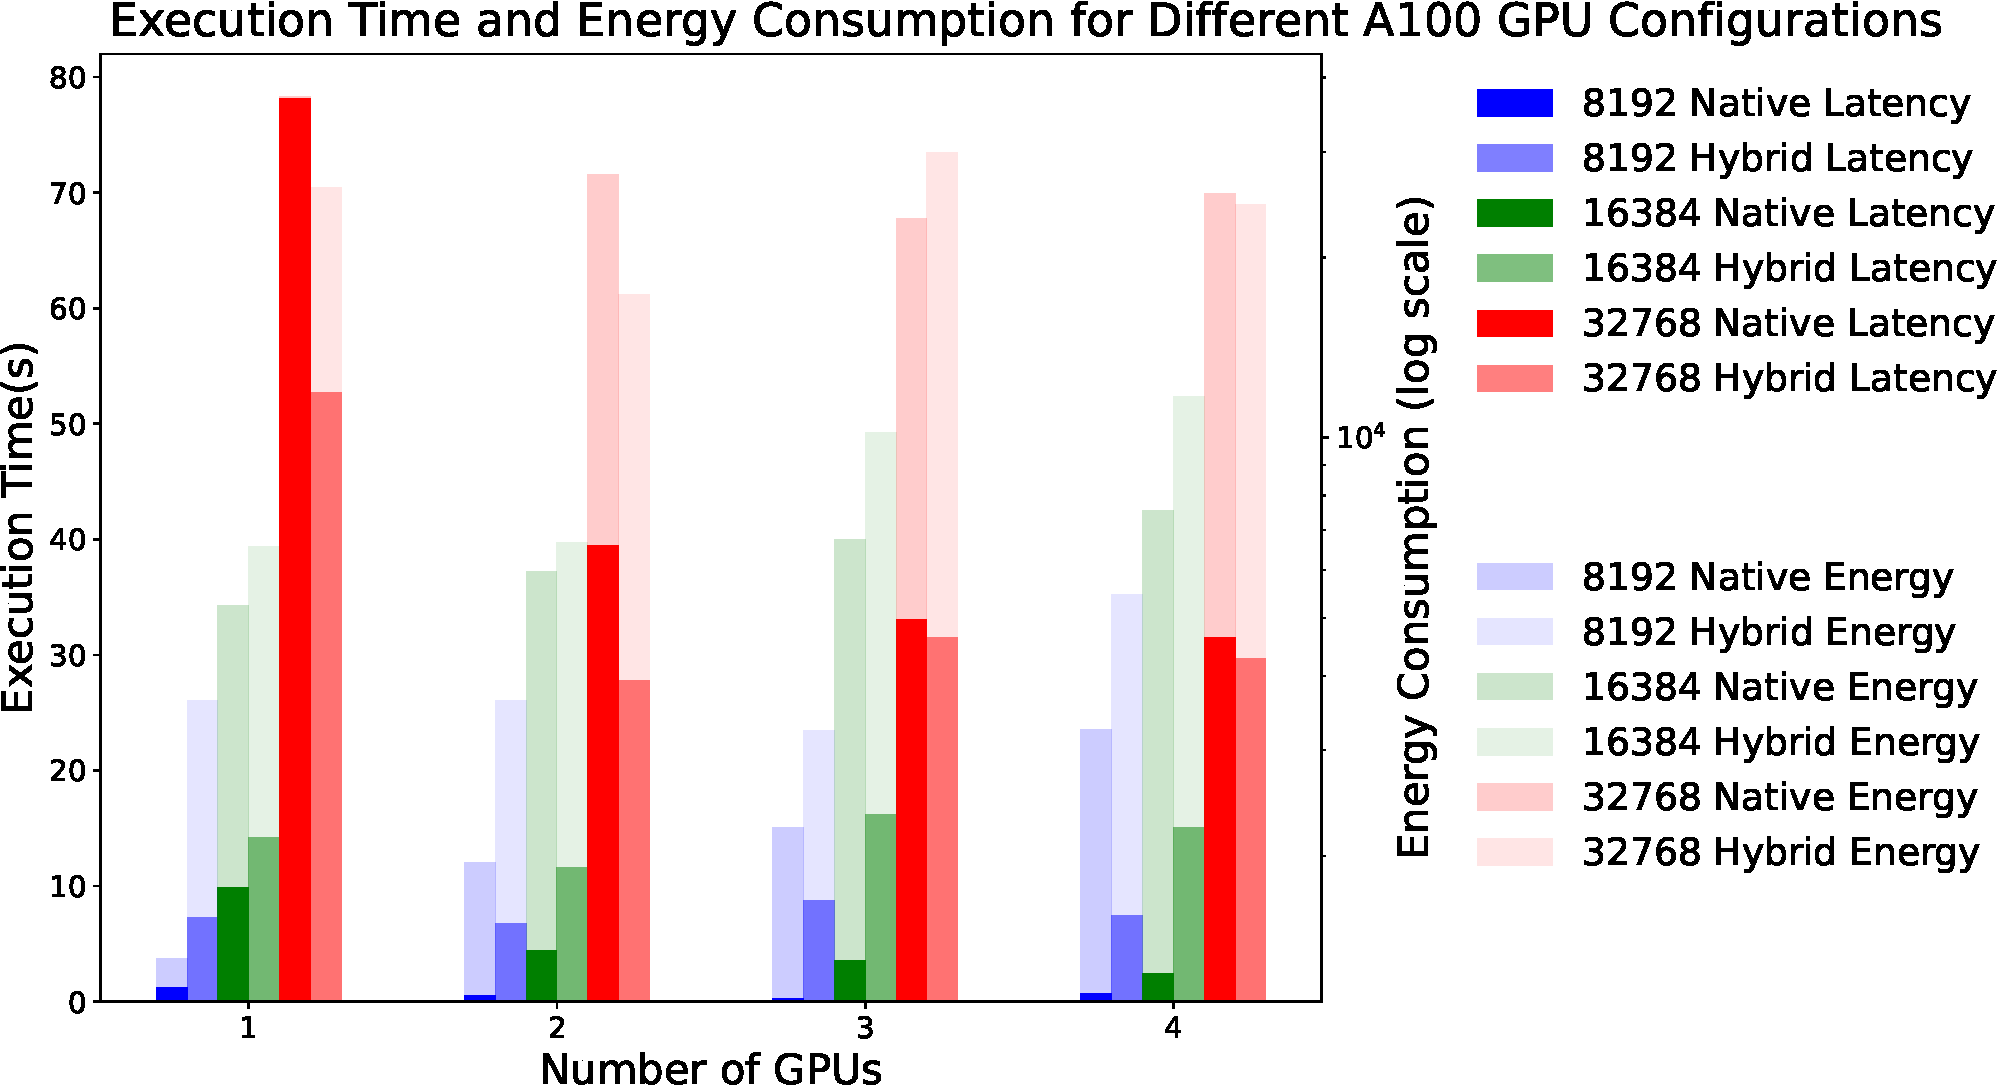
\includegraphics[width=\linewidth, height=5cm]{Images/a100-crop.pdf}
        
    \end{minipage} &
    \begin{minipage}{0.45\linewidth}
        \centering
        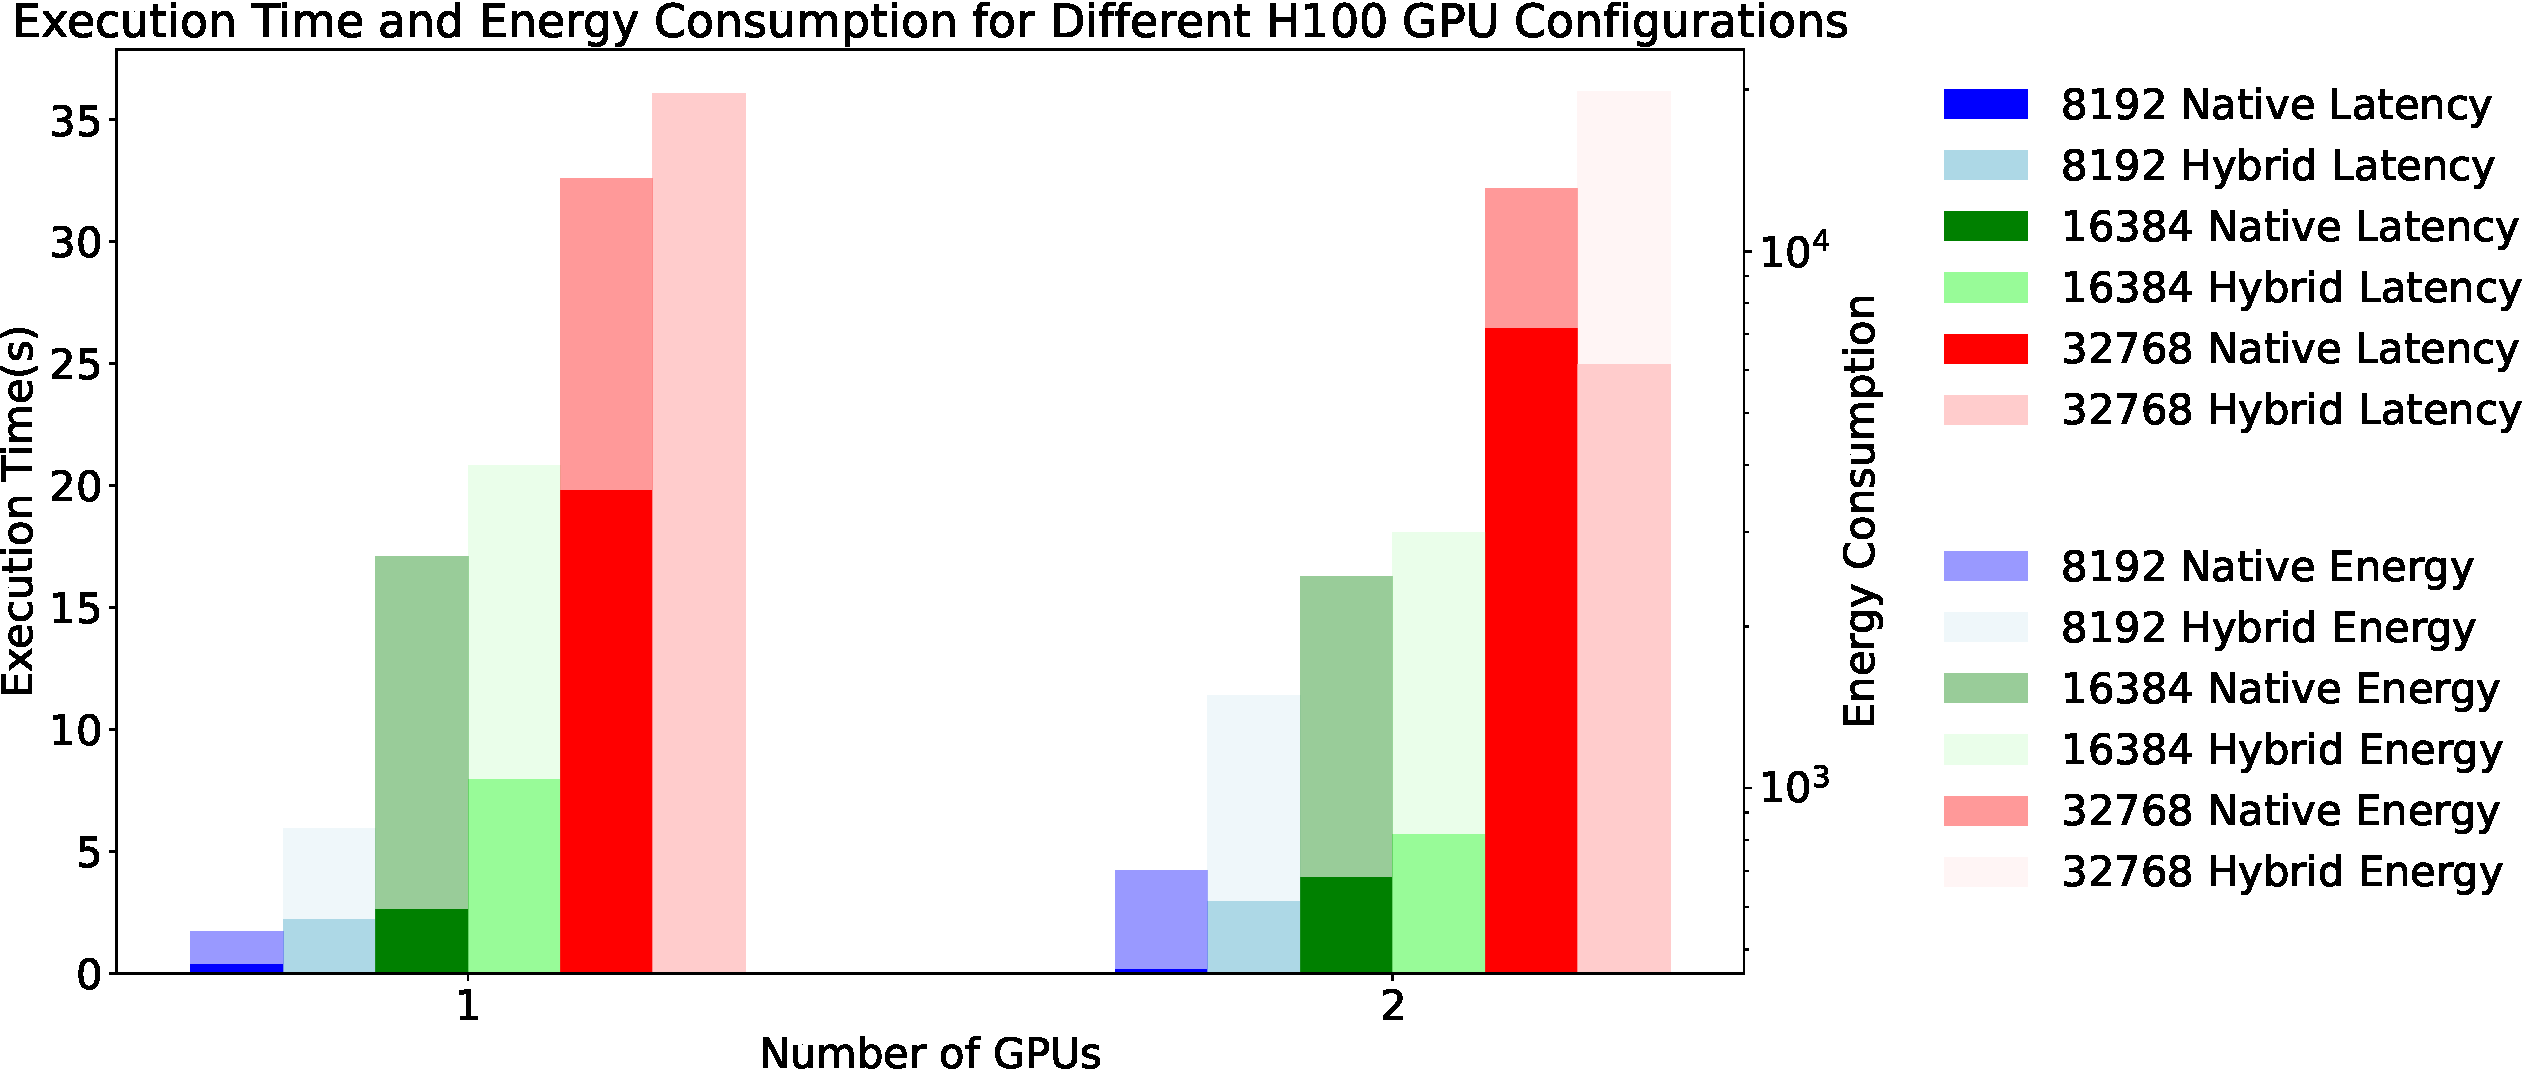
\includegraphics[width=\linewidth, height=5cm]{Images/h100-crop.pdf}
    \end{minipage} \\
\end{tabular}
\caption{Native CUDA-C vs. Augmented CUDA-C comparison on A100 and H100 GPU servers}
\label{fig:A100_H100_nat_vs_aug}
\end{figure*}

\begin{figure*}[htbp]
\centering
\begin{tabular}{cc}
    \begin{minipage}{0.45\linewidth}
        \centering
        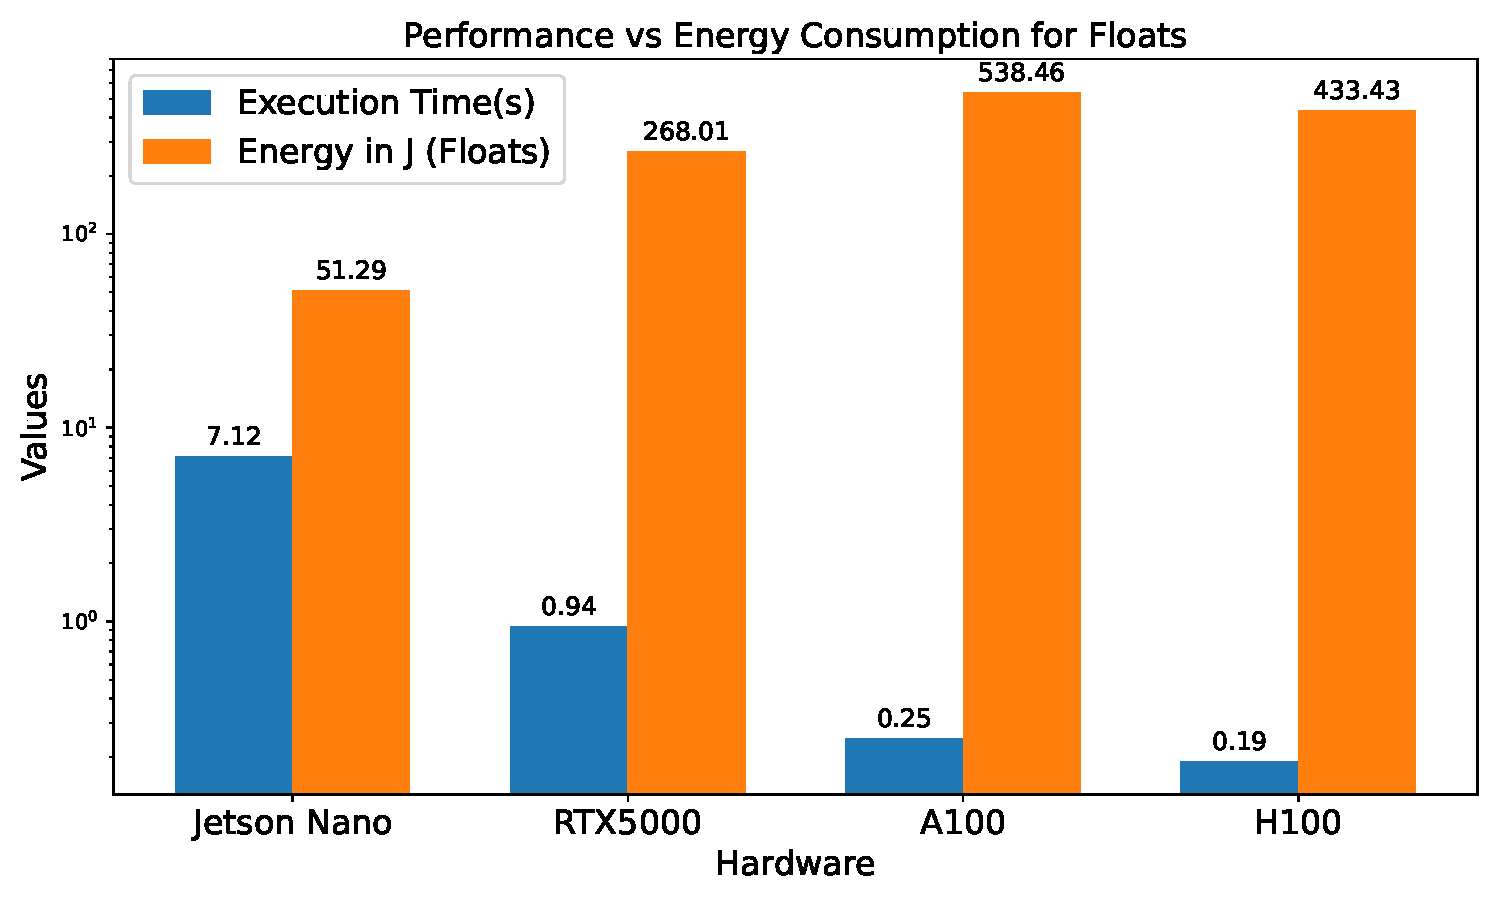
\includegraphics[width=\linewidth]{Images/cuda2.pdf}
    \end{minipage} &
    \begin{minipage}{0.45\linewidth}
        \centering
        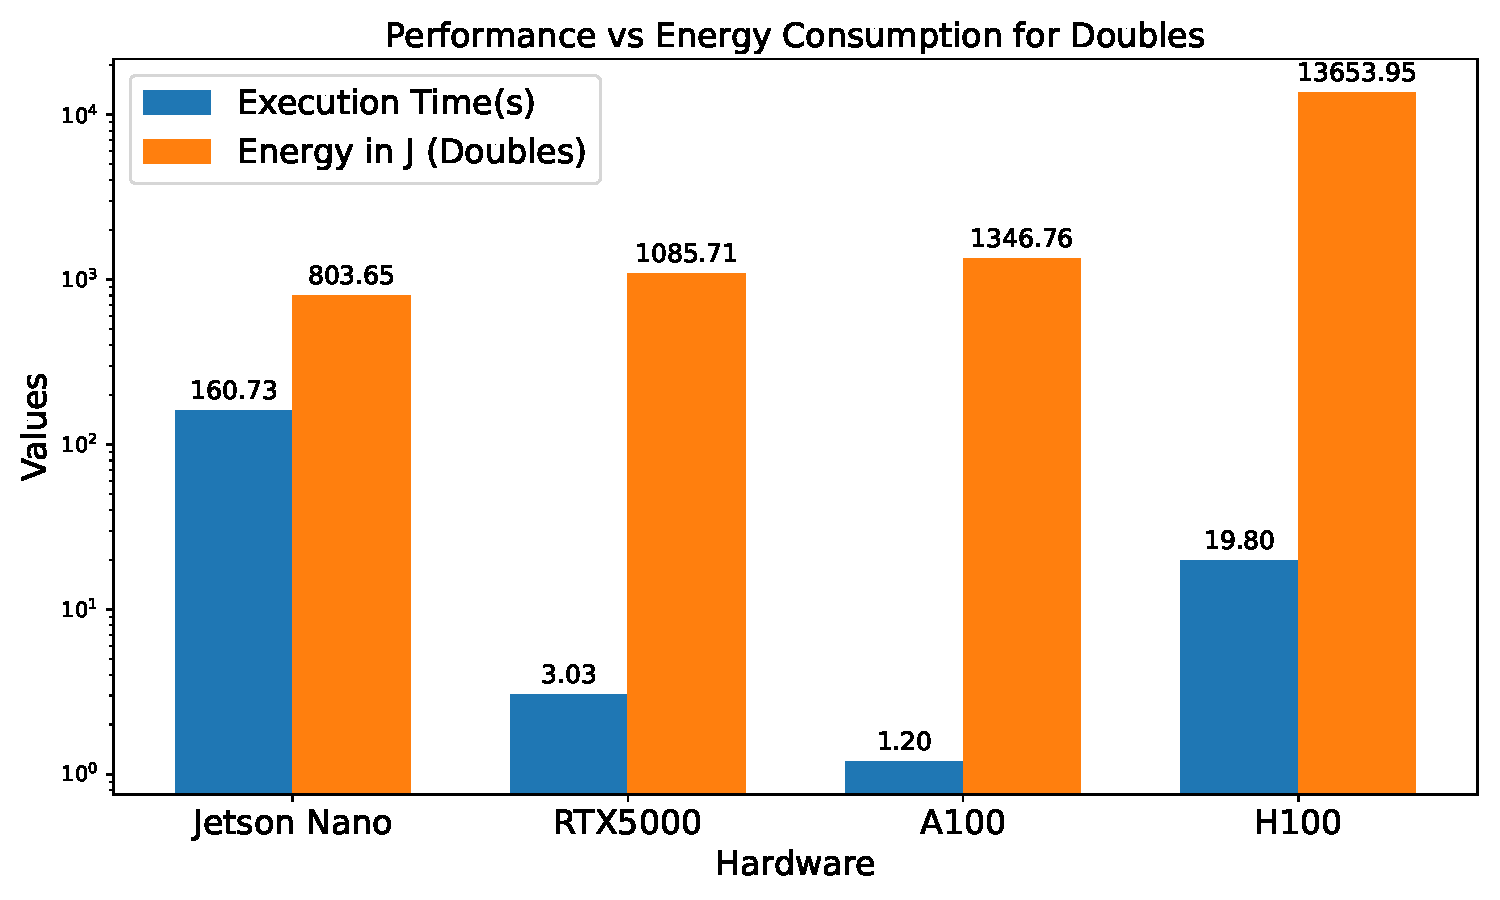
\includegraphics[width=\linewidth]{Images/cuda1.pdf}
    \end{minipage} \\
\end{tabular}
\caption{Performance and Energy consumption of Cuda codes on different Hardwares}
\label{fig:figcudaJNRTX}
\end{figure*}


\subsection{Discussion}

For most codes outside the numerical computing world, double-precision may be an overkill. Even single-precision \texttt{float} data may be over provisioning. In such scenarios, a latency vs. development speed or energy efficiency vs. development speed tradeoff would be more appropriate. Our study shows on multicore execution with \texttt{float} data, OpenMP (OMP) codes deliver almost the same level of performance as that with SIMD codes. In Figure~\ref{fig:3d}, the rhs part shows this result.  OMP codes are much easier to develop and compiler optimizations vectorize the code effectively. Also, we observe that tool-generated hybrid code augmented with AVX performs slightly better than the native code.  If high-precision is necessary, \texttt{double} inputs are to be considered. The lhs part of the Figure shows the results. 

 Figure~\ref{fig:3d} also shows the results with GPU execution. Executions on single and multiple-GPUs, with or without CuBLAS provided APIs, D2P augmented and native are shown. The left half of each part (lhs or rhs) in the figure shows this. We observe that GPU executions consume less energy compared to CPU executions. This is mostly because of the much lesser execution time (latency) on GPUs. It is interesting to note that executions on multiple GPUs consume less energy compared to executions on single GPU. This can be counter-intuitive at first but is due to the overall reduction in execution time  resulting from the distribution of workload on multiple GPUs. Also as expected, increased precision is associated with increased latency and energy consumption. 


In a win-win scenario, we see that tool assisted code implementation yields not only faster development speed but also faster execution. We see that the hybrid parallel code implementation for multi-GPU systems is not only performance portable but executes faster compared to native CUDA code.  Figure~\ref{fig:A100_H100_nat_vs_aug} shows the results.  Also, because of the reduced execution time, hybrid parallel code execution consumes lesser energy. D2P multigpu code was executed with 4 MPI ranks and the base case of the recursion had CUDA-kernel to distribute the workload across available GPU cards on the system. The native code was a plain CUDA code and had kernel to distribute the workload across available GPU cards. The executions were performed with varying number of GPU cards on RTX5000, A100, and H100 systems (Figure~\ref{fig:1} shows the results with RTX5000 card). We see that the hybrid parallel code outperformed native code on these systems for double precision numbers by achieving higher total memory throughput while having slightly lower compute throughput. There was no significant performance impact from this slight variation in compute throughput. Whereas for single  precision values, the native code outperformed the hybrid code in terms of memory and computation throughput. As a result, a similar behaviour as doubles is not seen in floats. Another interesting observation is that the difference in the latency between the cudaSgemm and CudasingleGPU implementations vanishes from 4k to 8k.To understand this behaviour, we profiled the codes using profilers mentioned in previous section. Through the profiled information, we found that the computational intensity of both codes almost doubles from 4k to 8k to 16k, and for 16k-sized matrices, we see that cudaSgemm executes faster than cudasingleGPU. From this, we infer that the Cuda library-based approach is beneficial for matrix sizes greater than or equal to 8k. We continue the discussion on GPU executions with a focus on energy consumption next.
%\begin{figure*}[h]
%   \centering
%   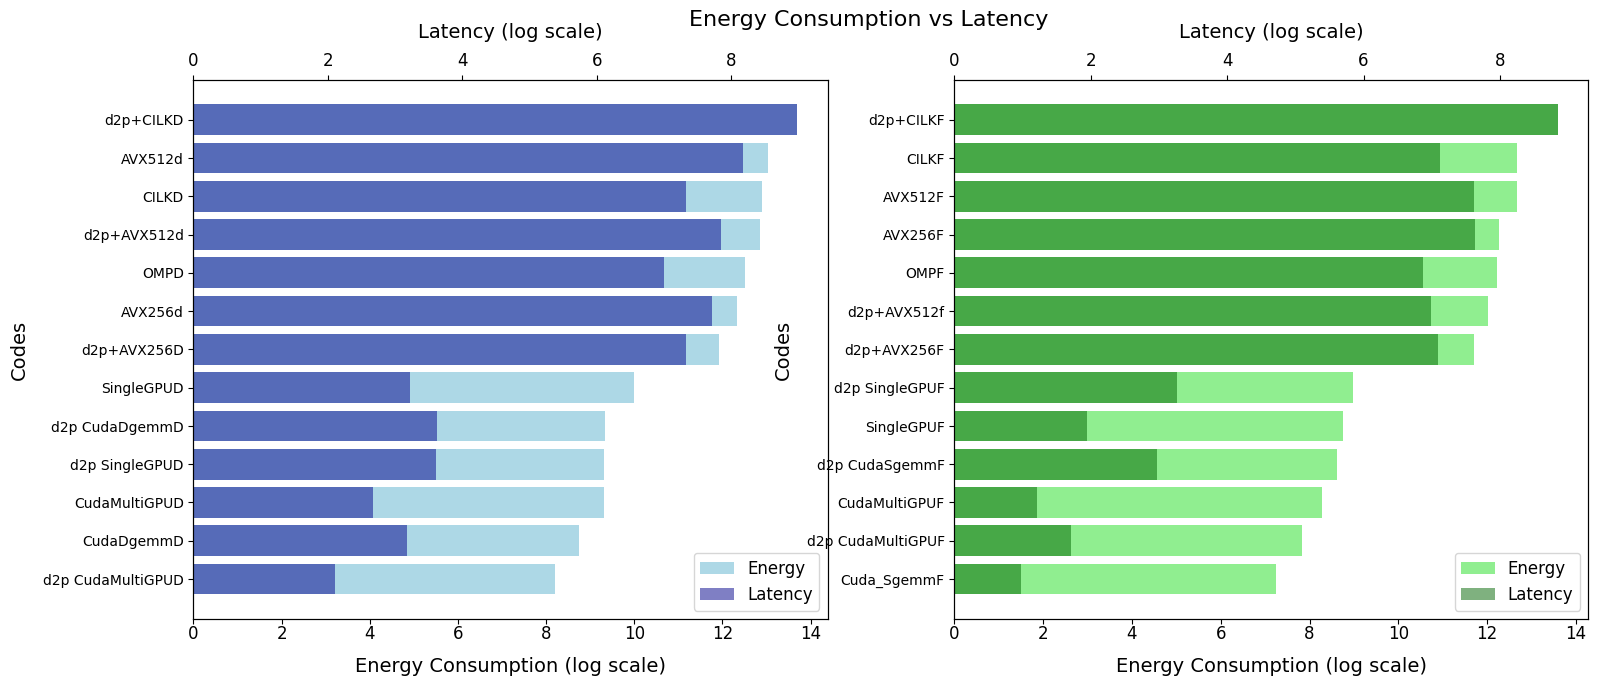
\includegraphics[width=0.8\textwidth]{2d dodgeplot1.png}
%    \caption{Consolidated Plot for easy analysis}
%    \label{fig:dodge}
%\end{figure*}



% For displaying results of next section on the same page
\begin{figure*}[ht]
\centering
\begin{tabular}{ccc}
    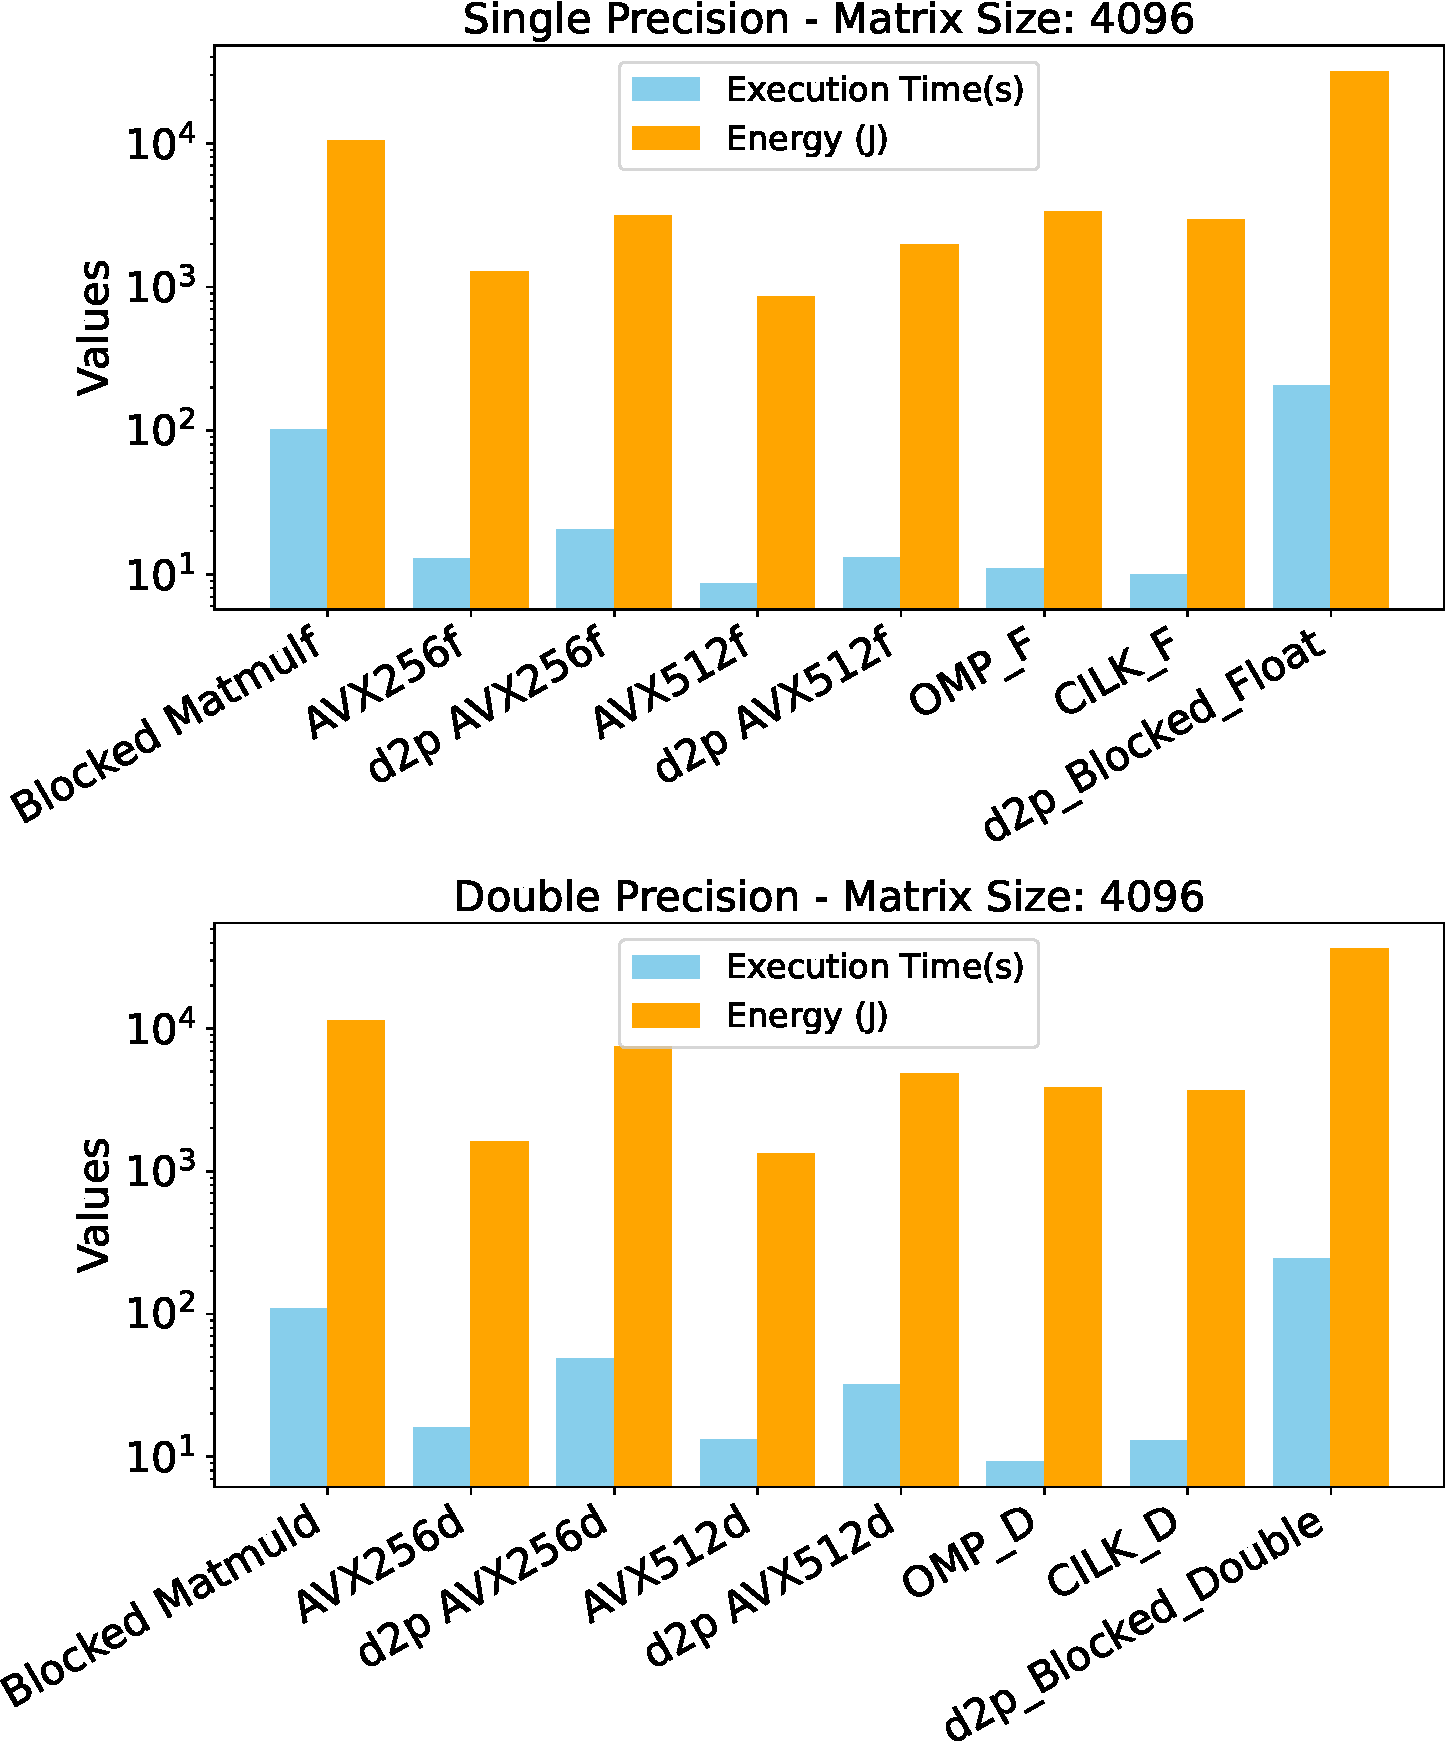
\includegraphics[width=0.32\linewidth,height=7cm]{Images/cpu4k-crop.pdf} &
    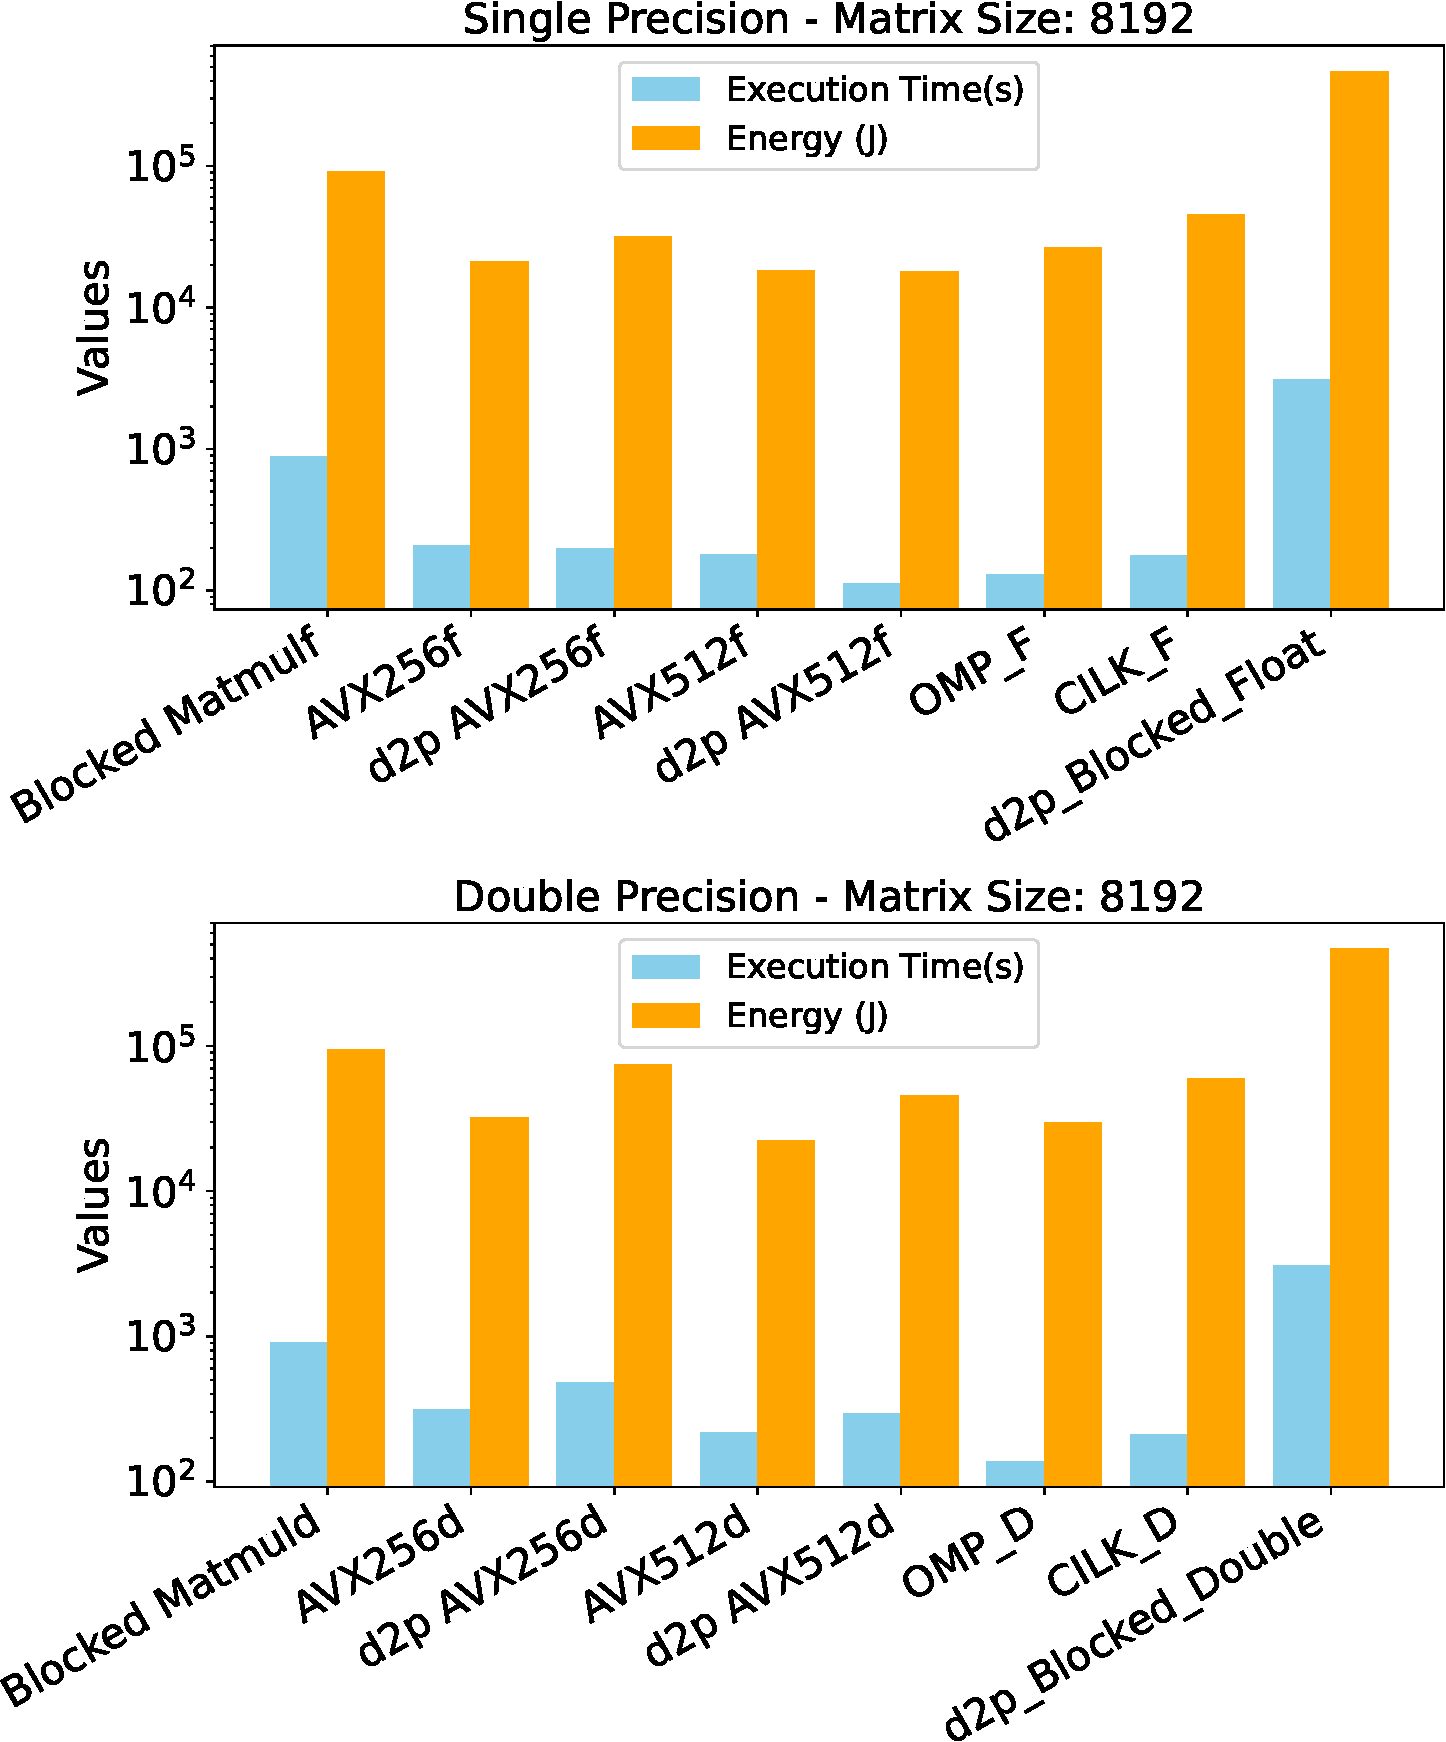
\includegraphics[width=0.32\linewidth,height=7cm]{Images/cpu8k-crop.pdf} &
    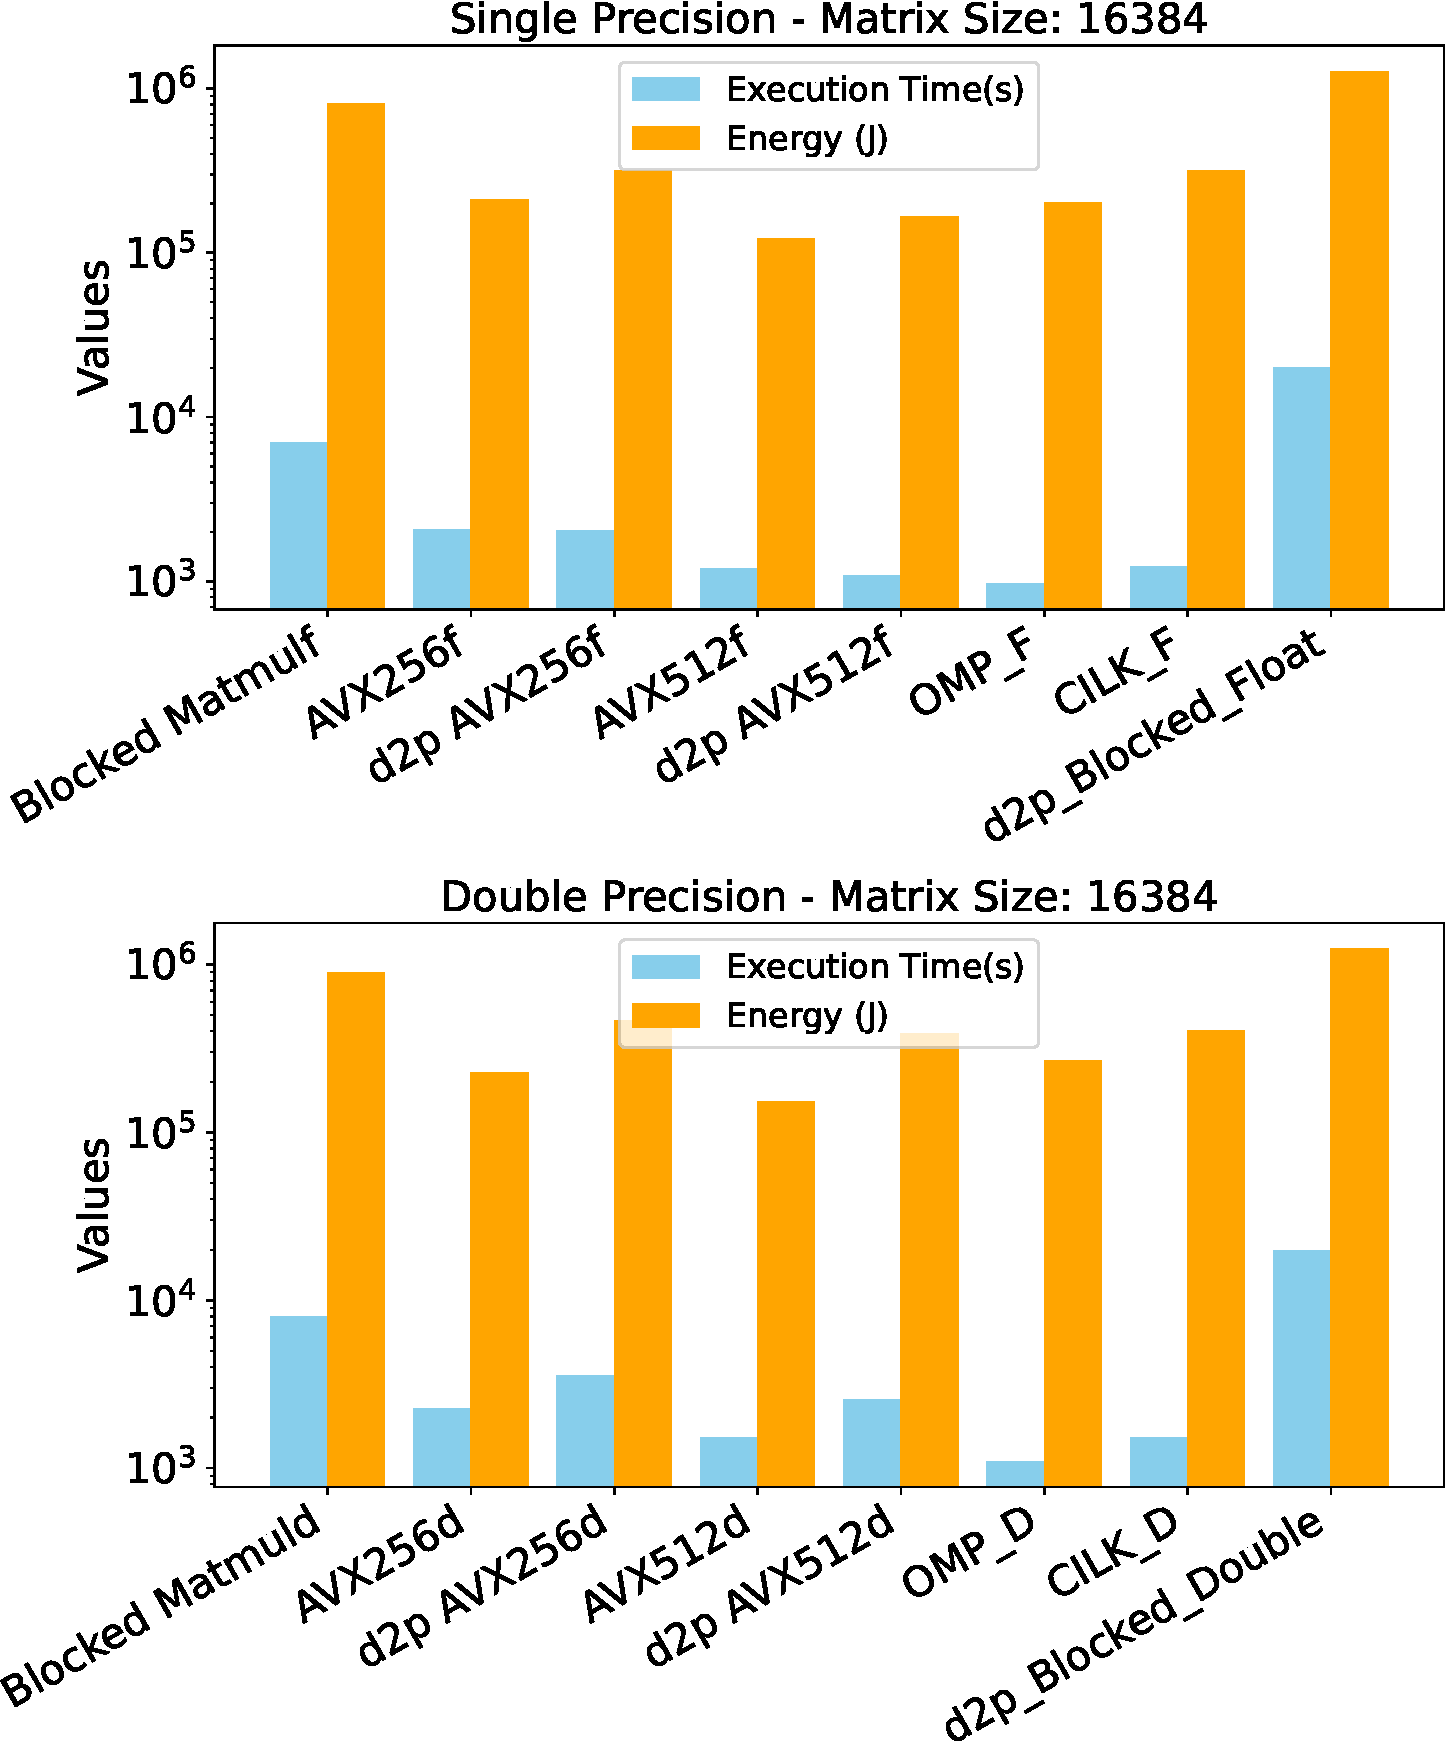
\includegraphics[width=0.32\linewidth,height=7cm]{Images/cpu16k-crop.pdf}\\ 
    (a) 4k & (b) 8k & (c) 16k \\
\end{tabular}
\caption{Performance characteristics on CPU cores for sizes 4k to 16k}
\label{fig:cpumulticore}
\end{figure*}




\begin{comment}
\begin{figure}[h!]
  \centering
  \includegraphics[width=1.0\linewidth]{A100.png}
  %\vspace{-0.8em}
  \caption{Native CUDA-C vs. Augmented CUDA-C comparison on A100 with matrix sizes scaling from 8k to 32k.}
  \label{fig:A100}
\end{figure}
\end{comment}



%\subsection{Experimental Analysis}
\paragraph{Energy consumption on GPUs and Jetson Nano} 
Figure~\ref{fig:figcudaJNRTX} shows the energy consumption when we execute native matrix-multiplication code with 8k input matrix size. We use a single GPU card on each of the GPU-servers in these experiments. The figure shows the data for both single- and double-precision inputs. With single-precision input data, Jetson Nano execution is 37$\times$ slower than the most powerful H100 GPU execution. In contrast, the Jetson Nano is energy efficient compared to H100 by 8.5$\times$. With double precision input data,  Jetson Nano code is slower by 48.7$\times$ compared to RTX100, 133$\times$ compared to A100, and only 8.4$\times$ compared to H100. We observe that H100 performance falls below that of A100 for double-precision data and are doing further study to understand the reason. Energy consumption-wise, Jetson Nano is 1.7$\times$ more efficient compared to the best performing A100 GPU for double-precision inputs. Beyond 8k input matrix sizes, we start seeing overflow in Jetson Nano. This experiment shows that in a scenario with lower precision requirement and no strict latency requirement, Jetson Nano can be very energy efficient when single-precision \texttt{float} data is chosen.    

%\input{Figures/Colab TPU results using TensorFlow and PyTorch}
\begin{figure*}[h]
    \centering
    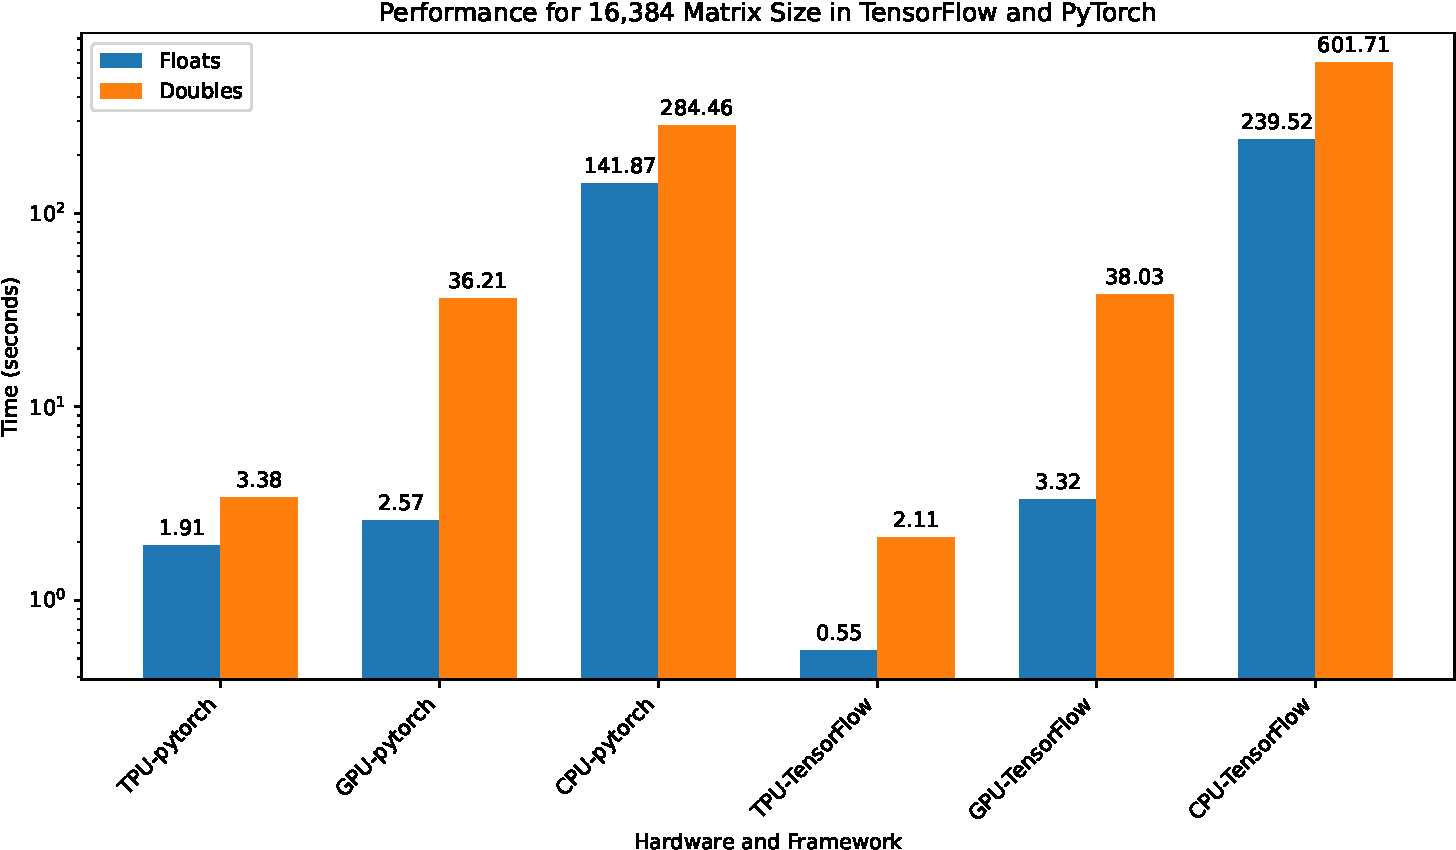
\includegraphics[width=0.75\textwidth]{Images/TF&Py-crop.pdf}
    \caption{Colab TPU results using TensorFlow and PyTorch}
    \label{fig:TPU}
\end{figure*}
\paragraph{TPU executions}
We explored TPU performance using TensorFlow and PyTorch for matrix multiplication on Google Colab, comparing it to GPU v4 and CPU for matrix sizes varying from 4k to 16k as before. Due to restricted hardware access, power consumption details were not available. For a 16k matrix, PyTorch showed that the TPU was 74x faster than the CPU and 1.2x faster than the GPU for single precision, and 84x faster than the CPU and 10x faster than the GPU for double precision. TensorFlow results indicated that the TPU was 6x faster than the GPU and 435x faster than the CPU for single precision, and 280x faster than the CPU and 18x faster than the GPU for double precision. The findings focus on  the trade-offs among latency and energy consumption in multi-GPU setups and the performance of TPUs for  matrix operations. Figure~\ref{fig:TPU} shows the results.

\paragraph{multicore execution on x86 and Arm}
We begin with multicore execution on x86 architectures. We have evaluated blocked (tiled), OMP, Cilk, AVX, AVX2, D2P with (tiled, AVX, and AVX2) variants on the RTX5000 system (we have named this system as RTX5000 but not used the GPU card in these experiments.). Figure~\ref{fig:cpumulticore} shows the details. 

As we increase the matrix size from 4k to 16k, the better-performing and energy-efficient programming model shifts. In the case of single precision, AVX512f is energy-efficient at 4k, whereas the OMP and D2P integrated with AVX512 become faster at 16k. On the other hand, for double precision, the OMP code constantly has lower latency, whereas  AVX512d remains energy-efficient across all matrix sizes. Figure~\ref{fig:armvsx86} shows the results of executing on Arm based instance on AWS. Figure~\ref{fig:arm} shows the trend observed on ARM systems, i.e., Native NEON code performs better than Hybrid NEON code for all the matrix sizes for single and extended precision.In figure \ref{fig:armvsx86}, observe that OMP and CILK codes on ARM perform better than x86.

We have also explored library-based methods like CBLAS and MKL implementations, where MKL outperformed with significantly better execution time and lower energy consumption than CBLAS.  We also implemented the hybrid implementations, d2p\_cblas and d2p\_MKL, which showed improved performance and energy consumption relative to CBLAS. However, they still are less efficient than MKL. The AVX-based implementations combined with Cilk or OpenMP, exhibited the highest execution times and energy consumption among all methods.  The table~\ref{tab:comparison} displays the detailed analysis for each implementation. Apart from the above methods, we have also leveraged Kokkos framework to explore performance portability aspect. We observed that KOKKOS introduces an abstraction overhead, which results in it being 2.3x slower than native CPU and 15x slower than native CUDA codes, it is discussed in detail in the \cite{kokkos}.

\begin{table}[htbp]
    %\centering
    $$
    \setlength{\tabcolsep}{2pt}
    \begin{tabular}{|c|c|c|}
        \hline
        \textbf{Codes} & \textbf{Execution Time (s)} & \textbf{Energy Consumed (J)} \\
        \hline
        CBLAS\_D      & 15.83   & 4753.77  \\
        MKL\_D        & 9.15    & 2452.98  \\
        d2p\_cblasD   & 14.82   & 3940.68  \\
        d2p\_MKLD     & 14.95   & 3953.05  \\
        AVX+ CILKD    & 39.83   & 12037.66 \\
        AVX+ OPENMPD  & 40.31   & 11156.25 \\
        \hline
    \end{tabular}
    $$
    \caption{Comparison of execution time and energy consumption across different implementations for 16k-sized matrices.}
    \label{tab:comparison}
\end{table}


Table~\ref{tab:co} displays the cost of ownership details.Traditionally, the cost of ownership is computed in dollars.In our study, we adopted a metric that is generally used in the semi-conductor industry : picoJoules per bit. Aiming to provide an estimation of the amount of energy spent per bit of computation. This metric provides a standardised approach that takes into account the various geographical representations and cost structures. Using this metric provides a common representation that is universally applicable for a comparison of energy efficiency across diverse regions. 
The data in Table~\ref{tab:co} shows that harnessing accelerators like the Jetson Nano and exploiting the benefits of multi-GPU setups offer higher energy efficiency. In contrast, other implementations like AVX-Native, CILK, and OMP have high energy consumption. Optimized implementations like D2p AVX substantially reduce energy usage.


%TODO:More explanation about Total cost of Ownership

\begin{figure}[htbp]
  \centering
  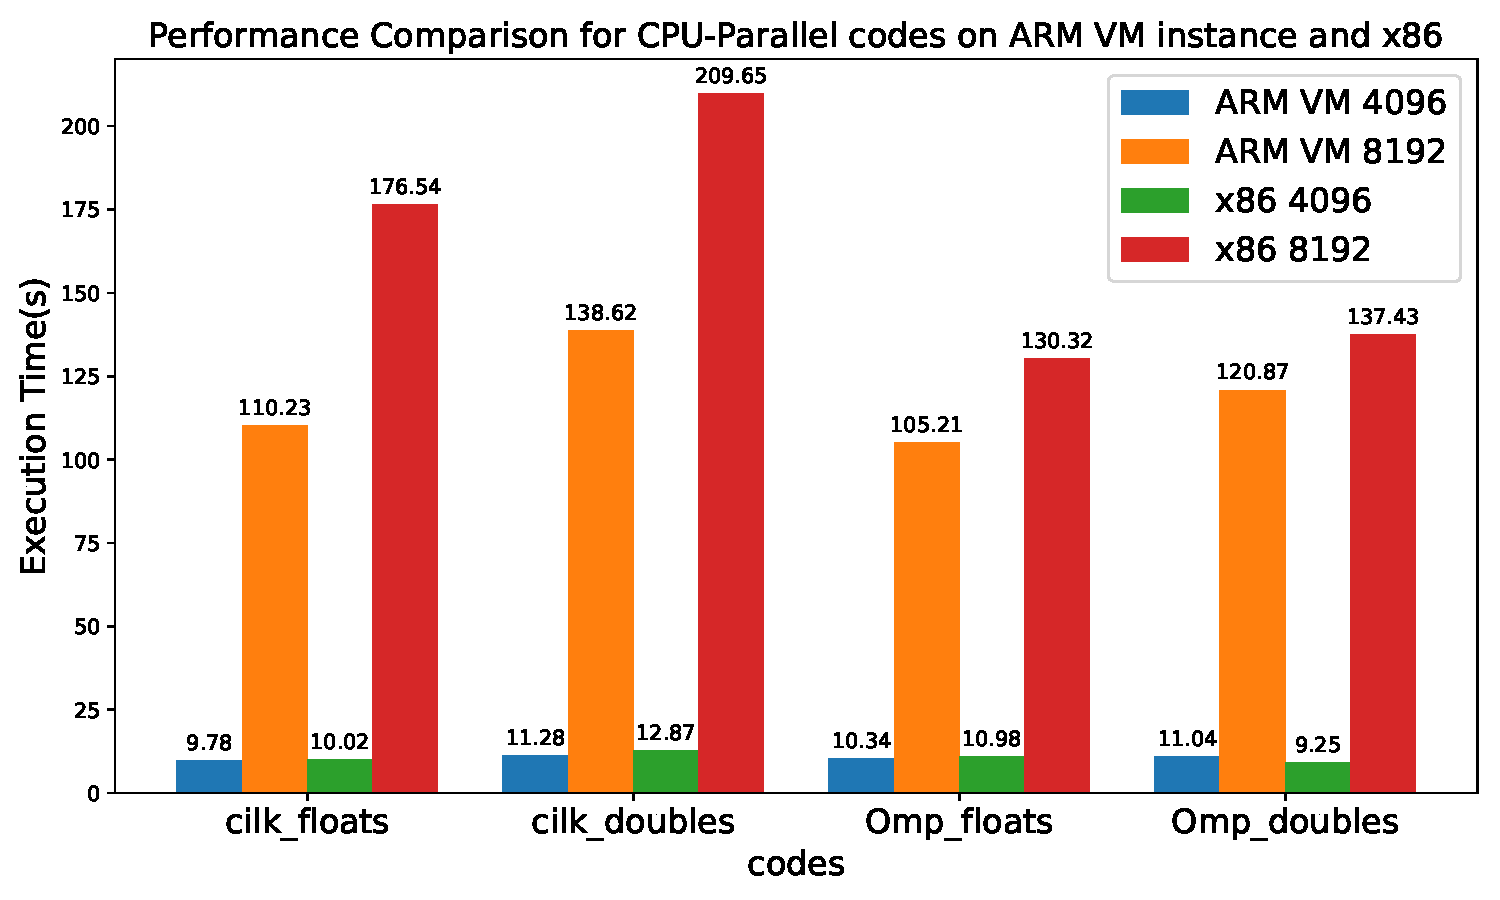
\includegraphics[width=1.0\linewidth]{Images/ARMvsx86.pdf}
  %\vspace{-0.8em}
  \caption{Performance of CPU Parallel codes on ARM vs x86.}
  \label{fig:armvsx86}
\end{figure}
%\begin{figure*}[ht]
\centering
\caption{Comparison of Single and Double Precision GPU Codes on RTX5000 and Jetson Nano}

\begin{subfigure}{0.45\linewidth}
    \centering
    \includegraphics[width=\linewidth]{Images/newRTXJNF.png}
    \caption{Single Precision 4k}
    \label{fig:RTXJNfloat4k}
\end{subfigure}
\hfill
\begin{subfigure}{0.45\linewidth}
    \centering
    \includegraphics[width=\linewidth]{Images/newRTXJNF8k.png}
    \caption{Single Precision 8k}
    \label{fig:RTXJNfloat8k}
\end{subfigure}

\begin{subfigure}{0.45\linewidth}
    \centering
    \includegraphics[width=\linewidth]{Images/newRTXJND.png}
    \caption{Double Precision 4k}
    \label{fig:RTXJNdouble4k}
\end{subfigure}
\hfill
\begin{subfigure}{0.45\linewidth}
    \centering
    \includegraphics[width=\linewidth]{Images/newRTXJND8k.png}
    \caption{Double Precision 8k}
    \label{fig:RTXJNdouble8k}
\end{subfigure}
\label{fig:gpu}
\end{figure*}

\input{Figures/Native Vs Hybrid using NEON intrinsics}

%\input{Figures/Latency-Energy Consumption trade-off for Multi-GPU on NVIDIA A100 & H100 GPUs}


\begin{figure*}[htbp]
\centering
\caption{Native Vs Hybrid using NEON intrinsics}
\begin{subfigure}{0.45\linewidth}
    \centering
    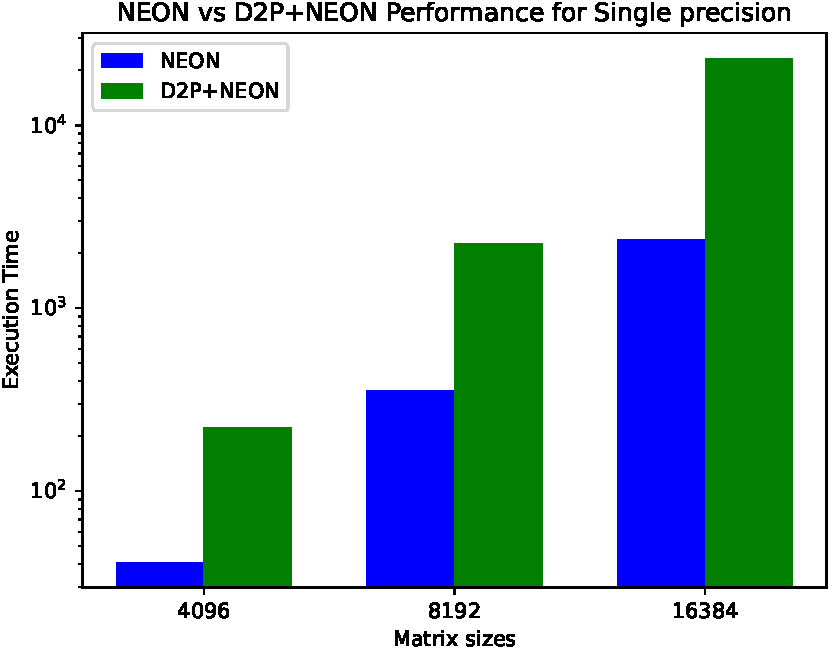
\includegraphics[width=0.90\linewidth]{Images/d2pvsNEONf-crop.pdf}
    \caption{Single precision}
    \label{fig:arm_float}
\end{subfigure}
\hfill
\begin{subfigure}{0.45\linewidth}
    \centering
    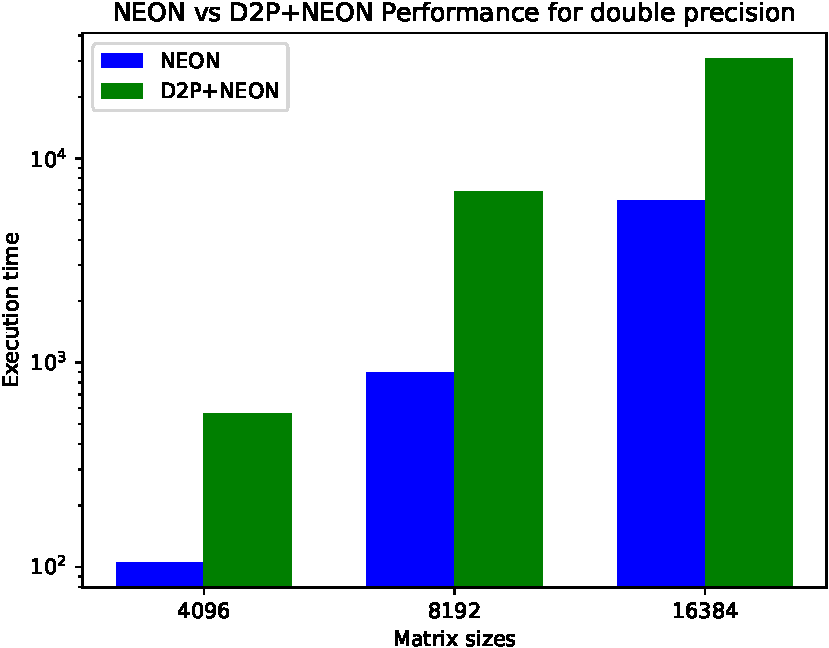
\includegraphics[width=0.90\linewidth]{Images/d2pvsNEONd-crop.pdf}
    \caption{Double precision}
    \label{fig:arm_double}
\end{subfigure}
\label{fig:arm}
\end{figure*}  


The performance peak percentages across the different hardware architectures display apparent differences in their ability to maximise efficiency as shown in Table \ref{tab:ppp}. The A100 demonstrates strong scalability in hybrid code, especially with multiple GPUs, reaching a peak of 24.47\% and outperforming its native counterpart. On the other hand, H100  performs well for native single-GPU execution, achieving 36.64\%, but it reduces for multiple gpus, indicating less scalability in multi-GPU setups. In contrast, the Quadro RTX 5000 performs poorly in single-GPU execution (3.14\%) but benefits significantly from hybrid parallelism in multi-GPU configurations, achieving 9.07\% peak performance. A common takeaway from these results is that hybrid parallelism yields better performance in multi-GPU setups, as seen with all the hardware, while single-GPU performance is maximised in native execution, especially with the H100.

As our future work, we will extend our experimentation on clusters with GPU nodes and power measurements on Arm based systems and TPUs.
\begin{table}[htbp]
$$
\begin{array}{|l|l|}
\hline \text {\textbf{Versions}} & \textbf{ picoJoules/bit } \\
\hline \text { D2p AVX } & 1019.98 \\
\hline \text { D2p cuda } & 69.51 \\
\hline \text { D2p Sgemm } & 66.88 \\
\hline \text { D2p multigpu } & 40.03 \\
\hline \text { OMP } & 1501.29 \\
\hline \text { CILK } & 2587.76 \\
\hline \text { Jetson Nano} & 2.91 \\
\hline \text { AVX-Native} & 6915.32 \\
\hline
\end{array}
\vspace{-0.25cm}
$$
\caption{Cost of ownership}
\label{tab:co}
\end{table}


\begin{table}[htbp]
\centering
\begin{tabular}{|c|c|c|c|}
\hline
\textbf{Hardware} & \textbf{GPUs} & \textbf{Native (\%)} & \textbf{Hybrid (\%)} \\ \hline
A100              & 1             & 9.29                 & 13.76                \\ \hline
A100              & 2             & 18.37                & 26.14                \\ \hline
A100              & 3             & 21.97                & 23.04                \\ \hline
A100              & 4             & 23.06                & 24.47                \\ \hline
H100              & 1             & 36.64                & 20.11                \\ \hline
H100              & 2             & 8.87                 & 9.40                 \\ \hline
Quadro RTX        & 1             & 3.136                & 2.125                \\ \hline
Quadro RTX        & 2             & 5.822                & 9.069                \\ \hline
\end{tabular}
\caption{Peak Performance Percentages for Native and Hybrid Codes on Different Hardware}
\label{tab:ppp}
\end{table}








\section{Related Work}
%This section explores different existing approaches to optimise Matrix-Mutliplication kernels.
%\subsection{Memory Hierarchy Optimisations}
Traditional approaches that exploited the memory hierarchy include~\cite{van1997summa,low2004api}. They aim at improving the data locality by blocking and loop interchange.
%\subsection{Library based solutions}
Earlier efforts in optimizing matrix multiplication kernels that have primarily focused on library development, are shown in various studies~\cite{anderson1999lapack, goto2008high, low2004api, choi1992scalapack,MKL} and for GPUs there are optimised frameworks such as~\cite{abdelfattah2016kblas}. 
%\subsection{Algorithmic Improvements}
Other studies, including \cite{fatahalian2004understanding, dorrance2014scalable, dalton2015optimizing, nagasaka2017high}, have implemented new algorithms to optimize sparse matrix-matrix and matrix-vector multiplication kernels on GPUs. On the other hand for dense matrix-vector computations we have have~\cite{fujimoto2008dense,nath2011optimizing}  Furthermore,  a GPU and CPU-GPU systems framework has been developed, as outlined in \cite{liu2015framework}. 
%\subsection{Exo-Compilation}
There are compiler and language approaches that address the optimization of the kernels. One of them is exo compilation~\cite{ikarashi2022exocompilation}, in which compiler backend decisions are externalised and are brought into the realm of the programmers. This approach, employs a  Python-like code that rewrites library functions into hardware-level optimised code. This approach is similar to that employed in domain-specific language Halide~\cite{ragan2013halide}, which mainly targets image processing kernels, where matrix-vector operations dominate. Halide targets single-node, multi-node, and GPU-based systems. 
%\subsection{Vectorization}
Vectorisation is also an approach to optimise the performance, some of the works include~\cite{tian2015effective} which presents effective vectorisation techniques on Xeon Phi processors.
%\subsection{Tools}
Tool based approaches reduce the programmer effort by doing automatic dependency inference, parallelism extraction, and/or code generation/execution~\cite{hegde2019d2p, van2009libflame}. ~\cite{hegde2019d2p} only targets Dynamic programming algorithms and ~\cite{van2009libflame} provides an API based approach and developers are required to re-engineer the code using the APIs.
Hierarchical tiling for improved superscalar performance~\cite{carter1995hierarchical} and automatic variable blocking for dense linear algebra algorithms~\cite{gustavson1997recursion} highlight the advanced techniques that improve the execution efficiency of matrix operations by optimising how data is accessed and stored in memory. Further research has been done in~\cite{chatterjee1999nonlinear} on nonlinear array layouts for hierarchical memory systems. Furthermore, an experimental comparison of cache-oblivious and cache-conscious programs demonstrates the benefits of these approaches in parallel algorithm design~\cite{yotov2007experimental}. The automatic generation of block-recursive codes, emphasizing memory optimization, is also studied in~\cite{ahmed2000automatic}.Some studies have compared the energy efficiency of GPUs with FPGAs \cite{mittal2014survey} and examined how the efficiency of matrix multiplication methods varies with the density of multi-GPU systems \cite{zhang2015matrix}. Besides, there is also study on performance evaluation on level-3 operations in CUBLAS \cite{barrachina2008evaluation}.
 Additionally, comparisons between FPGAs and GPUs for memory intensive and task that have less memory usage are shown in \cite{betkaoui2010comparing}.In addition, previous research on scientific and engineering subroutine libraries for vector processors has given important insights that guide modern optimization techniques~\cite{agarwal1989engineering}.



\section{Conclusions}
Our tool-generated implementation approach offers a simpler approach to achieve performance portability and energy efficiency across multiple cores, accelerators and GPU cards. Although domain experts may find it difficult at first to create a specification as input, we find that the recursive algorithms' close resemblance to the spec effectively overcomes this obstacle. Experimenting with various Hardware configurations, such as DNN accelerators and GPU-enabled single and multi-card servers, demonstrated the efficacy of our tool-based approach. Our work provides a peek into the energy consumption, latency, and speed of development to help developers deploy their matrix-multiplication based applications on an appropriate workhorse. 


\bibliographystyle{IEEEtran}
\bibliography{references}
\end{document}
